\documentclass[10pt,leqno]{article}
\usepackage[a4paper,margin=22mm,headheight=14pt]{geometry}
\usepackage{fontspec}
\setmainfont{Cambria}
\usepackage{amsmath,amssymb,amscd,mathtools}
\makeatletter
\renewcommand{\tagform@}[1]{\maketag@@@{\bfseries(#1)}}
\makeatother
\usepackage{unicode-math}
\setmathfont{Cambria Math}
\usepackage{graphicx,fancyhdr,microtype,seqsplit}
\graphicspath{{../assets/presentation_derivatives/}{./}}
\usepackage[hidelinks]{hyperref}
\setlength{\parindent}{0pt}
\setlength{\parskip}{.4em}
\setlength{\emergencystretch}{3em}
\allowdisplaybreaks
\pagestyle{fancy}\fancyhf{}
\fancyhead[L]{Pierre Deligne}
\fancyhead[R]{La conjecture de Weil. I}
\fancyfoot[C]{\thepage}
\begin{document}


\begin{center}{\Large\bfseries THE WEIL CONJECTURE. I}\par\medskip by PIERRE DELIGNE\end{center}

\phantomsection\label{physical-2}\noindent{\footnotesize Authority physical page 2; printed 273}\par\smallskip

\section*{CONTENTS}

\noindent 1. Grothendieck’s theory: cohomological interpretation of \(\mathrm{L}\)-functions\dotfill 273\par

\noindent 2. Grothendieck’s theory: Poincaré duality\dotfill 280\par

\noindent 3. The fundamental estimate\dotfill 283\par

\noindent 4. Lefschetz theory: local theory\dotfill 287\par

\noindent 5. Lefschetz theory: global theory\dotfill 289\par

\noindent 6. A rationality theorem\dotfill 294\par

\noindent 7. Completion of the proof of (1.7)\dotfill 298\par

\noindent 8. First applications\dotfill 301\par

\noindent In this article \(\mathrm{I}\) prove the Weil conjecture concerning the eigenvalues of Frobenius endomorphisms. \(\mathrm{A}\) precise statement is given in (1.6). I have tried to present the proof in as geometric and elementary a form as possible, and \(\mathrm{I}\) have included many reminders: only the results of §§ 3, 6, 7, and 8 are original.\par

\noindent In an article following this one, \(\mathrm{I}\) shall give various refinements of the intermediate results, and applications, among them the “hard” Lefschetz theorem (on iterated cup products by the cohomology class of a hyperplane section).\par

\noindent The text faithfully follows six lectures given at Cambridge in July 1973. I thank \(\mathrm{N}\). Katz for allowing me to use his notes.\par

\section*{1. Grothendieck’s theory: cohomological interpretation of \(\mathrm{L}\)-functions.}

\noindent \textbf{(1.1)} Let \(\mathrm{X}\) be a scheme of finite type over \(\mathbf{Z}\), let |\(\mathrm{X}|\) be the set of closed points of \(\mathrm{X}\), and, for \(x\in |\mathrm{X}|\), let \(\mathrm{N}(x)\) be the number of elements of the residue field \(k(x)\) of \(\mathrm{X}\) at \(x\). The Hasse-Weil zeta function of \(\mathrm{X}\) is\par

\begin{equation*}\begin{gathered}\zeta _{\mathrm{X}}(s) = \prod _{x\in |\mathrm{X}|} (1 -  \mathrm{N}(x)^{- s})^{- 1}\end{gathered}\tag{1.1.1}\end{equation*}

\noindent (this product converges absolutely for Re(\(s)\) sufficiently large). For \(\mathrm{X} = \operatorname{Spec}(\mathbf{Z}), \zeta _{\mathrm{X}}(s)\) is the Riemann zeta function.\par

\noindent We shall consider exclusively the case in which \(\mathrm{X}\) is a scheme over a finite field \(\mathbf{F}_{q}\).\par

\clearpage

\phantomsection\label{physical-3}\noindent{\footnotesize Authority physical page 3; printed 274}\par\smallskip

\noindent For \(x\in |\mathrm{X}|\), we shall write \(q_{x}\) rather than \(\mathrm{N}(x)\). Setting \(\operatorname{deg}(x)=[k(x):\mathbf{F}_{q}]\), we have \(q_{x}=q^{\operatorname{deg}(x)}\). It is useful to introduce the variable \(t=q^{- s}\). Put\par

\begin{equation*}\begin{gathered}\mathrm{Z}(\mathrm{X}; t) = \prod _{x\in |\mathrm{X}|} (1 -  t^{\operatorname{deg}(x)})^{- 1} ;\end{gathered}\tag{1.1.2}\end{equation*}

\noindent this infinite product converges for |\(t|\) sufficiently small, and\par

\begin{equation*}\begin{gathered}\zeta _{\mathrm{X}}(s) = \mathrm{Z}(\mathrm{X}; q^{- s}).\end{gathered}\tag{1.1.3}\end{equation*}

\noindent \textbf{(1.2)} Dwork (On the rationality of the zeta function of an algebraic variety, \emph{Amer. J. Math.}, 82, 1960, p. 631-648) and Grothendieck ([1] and SGA 5) proved that \(\mathrm{Z}(\mathrm{X},t)\) is a rational function of \(t\).\par

\noindent For Grothendieck, this is a corollary of general results in \(\ell \)-adic cohomology (\(\ell \) denotes a prime number different from the characteristic \(p\) of \(\mathbf{F}_{q})\). These furnish a cohomological interpretation of the zeros and poles of \(\mathrm{Z}(\mathrm{X};t)\), and a functional equation when \(\mathrm{X}\) is proper and smooth. Dwork’s methods are \(p\)-adic. For \(\mathrm{X}\) a nonsingular hypersurface in projective space, they likewise furnished a cohomological interpretation of the zeros and poles, and the functional equation. They inspired the crystalline theory of Grothendieck and Berthelot, which, for \(\mathrm{X}\) proper and smooth, furnishes a \(p\)-adic cohomological interpretation of the zeros and poles, and the functional equation. Building on ideas of Washnitzer, Lubkin created a variant of this theory, valid only for \(\mathrm{X}\) proper, smooth, and liftable to characteristic zero (A \(p\)-adic proof of Weil’s conjectures, \emph{Ann. of Math.}, 87, 1968, p. 105-255).\par

\noindent We shall make essential use of Grothendieck’s results and recall them below.\par

\noindent \textbf{(1.3)} Let \(\mathrm{X}\) be an algebraic variety over an algebraically closed field \(k\) of characteristic \(p\), i.e. a separated scheme of finite type over \(k\). We do not exclude the case \(p=0\). For every prime \(\ell \ne p\), Grothendieck defined \(\ell \)-adic cohomology groups \(\mathrm{H}^{i}(\mathrm{X},\mathbf{Q}_{\ell })\). He also defined cohomology groups with proper support \(\mathrm{H}_{c}^{i}(\mathrm{X},\mathbf{Q}_{\ell })\). For \(\mathrm{X}\) proper, the two coincide. The \(\mathrm{H}_{c}^{i}(\mathrm{X},\mathbf{Q}_{\ell })\) are finite-dimensional vector spaces over \(\mathbf{Q}_{\ell }\), and vanish for \(i>2 \operatorname{dim}(\mathrm{X})\).\par

\noindent \textbf{(1.4)} Let \(\mathrm{X}_{0}\) be an algebraic variety over \(\mathbf{F}_{q}\), let \(\overline{\mathbf{F}}_{q}\) be an algebraic closure of \(\mathbf{F}_{q}\), and let \(\mathrm{X}\) be the algebraic variety over \(\overline{\mathbf{F}}_{q}\) obtained from \(\mathrm{X}_{0}\) by extension of scalars from \(\mathbf{F}_{q}\) to \(\overline{\mathbf{F}}_{q}\). In the language of Weil or Shimura, one would express this situation as: “Let \(\mathrm{X}\) be an algebraic variety defined over \(\mathbf{F}_{q}\).” Let \(\mathrm{F}:\mathrm{X}\longrightarrow \mathrm{X}\) be the Frobenius morphism; it sends a point with coordinates \(x\) to the point with coordinates \(x^{q}\); in other words, for \(\mathrm{U}_{0} a\) Zariski-open subset of \(\mathrm{X}_{0}\) defining an open subset \(\mathrm{U}\) of \(\mathrm{X}\), one has \(\mathrm{F}^{- 1}(\mathrm{U})=\mathrm{U}\); for \(x\in \mathrm{H}^{0}(\mathrm{U}_{0},\mathcal{O})\), one has \(\mathrm{F}^{*}x=x^{q}\). Identify the set |\(\mathrm{X}|\) of closed points of \(\mathrm{X}\) with \(\mathrm{X}_{0}(\overline{\mathbf{F}}_{q})\) (the set \(\operatorname{Hom}_{\mathbf{F}_{q}}(\operatorname{Spec}(\overline{\mathbf{F}}_{q}),\mathrm{X}_{0})\) of points of \(\mathrm{X}_{0}\) with coordinates in \(\overline{\mathbf{F}}_{q})\), and let\par

\clearpage

\phantomsection\label{physical-4}\noindent{\footnotesize Authority physical page 4; printed 275}\par\smallskip

\noindent \(\varphi \in \operatorname{Gal}(\overline{\mathbf{F}}_{q}/\mathbf{F}_{q})\) be the Frobenius substitution: \(\varphi (x)=x^{q}\). The action of \(\mathrm{F}\) on |\(\mathrm{X}|\) identifies with the action of \(\varphi \) on \(\mathrm{X}_{0}(\overline{\mathbf{F}}_{q})\). Consequently:\par

\noindent a) The set \(\mathrm{X}^{\mathrm{F}}\) of closed points of \(\mathrm{X}\) fixed by \(\mathrm{F}\) identifies with the set \(\mathrm{X}_{0}(\mathbf{F}_{q})\subset \mathrm{X}_{0}(\overline{\mathbf{F}}_{q})\) of points of \(\mathrm{X}\) defined over \(\mathbf{F}_{q}\). This simply expresses that, for \(x\in \overline{\mathbf{F}}_{q}, x\in \mathbf{F}_{q} \Leftrightarrow  x^{q}=x\).\par

\noindent \(b)\) Likewise, the set \(\mathrm{X}^{\mathrm{F}^{n}}\) of closed points of \(\mathrm{X}\) fixed by the \(n\)-th iterate of \(\mathrm{F}\) identifies with \(\mathrm{X}_{0}(\mathrm{F}_{q^{n}})\).\par

\noindent \(c)\) The set |\(\mathrm{X}_{0}|\) of closed points of \(\mathrm{X}_{0}\) identifies with the set |\(\mathrm{X}|_{\mathrm{F}}\) of \(\mathrm{F}\)-orbits (or \(\varphi \)-orbits) in |\(\mathrm{X}|\). The degree \(\operatorname{deg}(x)\) of \(x\in |\mathrm{X}_{0}|\) is the number of elements in the corresponding orbit.\par

\noindent \(d)\) From \(b)\) and \(c)\) one obtains the formula\par

\begin{equation*}\begin{gathered}\# \mathrm{X}^{\mathrm{F}^{n}} = \# \mathrm{X}_{0}(\mathrm{F}_{q^{n}}) = \sum _{\operatorname{deg}(x)|n} \operatorname{deg} x\end{gathered}\tag{1.4.1}\end{equation*}

\noindent (for \(x\in |\mathrm{X}_{0}|\) and \(\operatorname{deg}(x)|n, x\) defines \(\operatorname{deg}(x)\) points with coordinates in \(\mathrm{F}_{q^{n}}\), all conjugate over \(\mathbf{F}_{q})\).\par

\noindent \textbf{(1.5)} The morphism \(\mathrm{F}\) is finite, hence in particular proper. It therefore induces maps\par

\begin{equation*}\begin{gathered}\mathrm{F}^{*} : \mathrm{H}_{c}^{i}(\mathrm{X},\mathbf{Q}_{\ell }) \longrightarrow  \mathrm{H}_{c}^{i}(\mathrm{X},\mathbf{Q}_{\ell }).\end{gathered}\end{equation*}

\noindent Grothendieck proved the Lefschetz formula\par

\begin{equation*}\begin{gathered}\# \mathrm{X}^{\mathrm{F}} = \sum _{i} (- 1)^{i} \operatorname{Tr}(\mathrm{F}^{*},\mathrm{H}_{c}^{i}(\mathrm{X},\mathbf{Q}_{\ell }));\end{gathered}\end{equation*}

\noindent the right-hand side, \emph{a priori} an \(\ell \)-adic number, is an integer and equals the left-hand side. Such a formula is reasonable only because dF=0, even at infinity (\(\mathrm{X}\) is not assumed proper); the relation dF=0 implies that the fixed points of \(\mathrm{F}\) have multiplicity one.\par

\noindent An analogous formula holds for the iterates of \(\mathrm{F}\):\par

\begin{equation*}\begin{gathered}\# \mathrm{X}^{\mathrm{F}^{n}} = \# \mathrm{X}_{0}(\mathrm{F}_{q^{n}}) = \sum _{i} (- 1)^{i} \operatorname{Tr}(\mathrm{F}^{*n},\mathrm{H}_{c}^{i}(\mathrm{X},\mathbf{Q}_{\ell })).\end{gathered}\tag{1.5.1}\end{equation*}

\noindent Take the logarithmic derivative of (1.1.2):\par

\begin{equation*}\begin{aligned}
t\frac{d}{dt}\log\mathrm Z(\mathrm X_0,t)&=\frac{t\frac{d}{dt}\mathrm Z(\mathrm X_0,t)}{\mathrm Z(\mathrm X_0,t)}
=\sum_{x\in|\mathrm X_0|}-\frac{-\deg(x)t^{\deg(x)}}{1-t^{\deg(x)}}\\
&=\sum_{x\in|\mathrm X_0|}\sum_{n>0}\deg(x)t^{n\deg(x)}
\underset{(1.4.1)}{=}\sum_n\#\mathrm X_0(\mathbf F_{q^n})\cdot t^n.
\end{aligned}\tag{1.5.2}\end{equation*}

\noindent For an endomorphism \(\mathrm{F}\) of a vector space \(\mathrm{V}\), one has the following identity of formal series:\par

\begin{equation*}\begin{gathered}t\cdot \frac{d}{dt} \operatorname{log}(\operatorname{det}(1- \mathrm{F}t,\mathrm{V})^{- 1}) = \sum _{n>0} \operatorname{Tr}(\mathrm{F}^{n},\mathrm{V})t^{n}\end{gathered}\tag{1.5.3}\end{equation*}

\clearpage

\phantomsection\label{physical-5}\noindent{\footnotesize Authority physical page 5; printed 276}\par\smallskip

\noindent (check this for \(\operatorname{dim}(\mathrm{V})=1\), and observe that both sides are additive in \(\mathrm{V}\) in a short exact sequence). Substituting (1.5.1) into (1.5.2) and applying (1.5.3), one obtains\par

\begin{equation*}\begin{gathered}t\cdot \frac{d}{dt} \operatorname{log} \mathrm{Z}(\mathrm{X}_{0},t) \\ = \sum _{i} (- 1)^{i} t\cdot \frac{d}{dt} \operatorname{log} \operatorname{det}(1- \mathrm{F}^{*}t,\mathrm{H}_{c}^{i}(\mathrm{X},\mathbf{Q}_{\ell }))^{- 1},\end{gathered}\end{equation*}

\noindent hence\par

\begin{equation*}\begin{gathered}\mathrm{Z}(\mathrm{X}_{0},t) = \prod _{i} \operatorname{det}(1- \mathrm{F}^{*}t,\mathrm{H}_{c}^{i}(\mathrm{X},\mathbf{Q}_{\ell }))^{(- 1)^{i+1}}.\end{gathered}\tag{1.5.4}\end{equation*}

\noindent The right-hand side is an element of \(\mathbf{Q}_{\ell }(t)\). The formula states that its Taylor expansion at \(t=0\), \emph{a priori} a formal series in \(\mathbf{Q}_{\ell }[[t]]\) with constant term one, belongs to \(\mathbf{Z}[[t]]\) and equals the left-hand side, itself also regarded as a formal series in \(t\). This is Grothendieck’s cohomological interpretation of the function \(\mathrm{Z}\).\par

\noindent Our principal result is the following.\par

\noindent \emph{Theorem} \textbf{(1.6)}. — {\itshape Let \(\mathrm{X}_{0}\) be a nonsingular (= smooth) projective variety over \(\mathbf{F}_{q}\). For every \(i\), the characteristic polynomial \(\operatorname{det}(t\cdot 1- \mathrm{F}^{*},\mathrm{H}^{i}(\mathrm{X},\mathbf{Q}_{\ell }))\) has integer coefficients independent of \(\ell  (\ell \ne p)\). The complex roots \(\alpha \) of this polynomial (the complex conjugates of the eigenvalues of \(\mathrm{F}^{*})\) have absolute value |\(\alpha |=q^{i/2}\).}\par

\noindent We first show that (1.6) follows from the apparently weaker result below.\par

\noindent \emph{Lemma} \textbf{(1.7)}. — {\itshape For every \(i\) and every \(\ell \ne p\), the eigenvalues of the endomorphism \(\mathrm{F}^{*}\) of \(\mathrm{H}^{i}(\mathrm{X},\mathbf{Q}_{\ell })\) are algebraic numbers all of whose complex conjugates \(\alpha \) have absolute value |\(\alpha |=q^{i/2}\).}\par

\noindent Proof that (1.7) implies (1.6). — Regard \(\mathrm{Z}(\mathrm{X}_{0},t)\) as a formal series with constant term 1, an element of \(\mathbf{Z}[[t]]: \mathrm{Z}(\mathrm{X}_{0},t)=\sum _{n} a_{n} t^{n}\). By (1.5.3), the image of \(\mathrm{Z}(\mathrm{X}_{0},t)\) in \(\mathbf{Q}_{\ell }[[t]]\) is the Taylor expansion of a rational function. This means that, for \(\mathrm{N}\) and \(\mathrm{M}\) sufficiently large (at least the degrees of the numerators and denominators), the Hankel determinants\par

\begin{equation*}\begin{gathered}\mathrm{H}_{k} = \operatorname{det}((a_{i+j+k})_{0\leq i,j\leq \mathrm{M}})    (k>\mathrm{N})\end{gathered}\end{equation*}

\noindent vanish. This vanishing holds in \(\mathbf{Q}_{\ell }\) if and only if it holds in \(\mathbf{Q}\); therefore \(\mathrm{Z}(\mathrm{X}_{0},t)\) is the Taylor expansion of an element of \(\mathbf{Q}(t)\). In other words,\par

\begin{equation*}\begin{gathered}\mathrm{Z}(\mathrm{X}_{0},t) \in  \mathbf{Z}[[t]] \cap  \mathbf{Q}_{\ell }(t) \subset  \mathbf{Q}(t).\end{gathered}\end{equation*}

\noindent Write \(\mathrm{Z}(\mathrm{X}_{0},t)=\mathrm{P}/\mathrm{Q}\), with \(\mathrm{P},\mathrm{Q}\in \mathbf{Z}[t]\) relatively prime and with positive constant terms. By a lemma of Fatou, the fact that \(\mathrm{Z}(\mathrm{X}_{0},t)\) belongs to \(\mathbf{Z}[[t]]\) and has constant term one implies that the constant terms of \(\mathrm{P}\) and \(\mathrm{Q}\) are 1. Put\par

\begin{equation*}\begin{gathered}\mathrm{P}_{i}(t)=\operatorname{det}(1- \mathrm{F}^{*}t,\mathrm{H}^{i}(\mathrm{X},\mathbf{Q}_{\ell })).\end{gathered}\end{equation*}

\clearpage

\phantomsection\label{physical-6}\noindent{\footnotesize Authority physical page 6; printed 277}\par\smallskip

\noindent By hypothesis (1.7), the \(\mathrm{P}_{i}\) are pairwise relatively prime. The right-hand side of (1.5.4) is therefore in reduced form, and\par

\begin{equation*}\begin{gathered}\mathrm{P}(t) = \prod _{i \text{odd}} \mathrm{P}_{i}(t) \\ \mathrm{Q}(t) = \prod _{i \text{even}} \mathrm{P}_{i}(t).\end{gathered}\end{equation*}

\noindent Let \(\mathrm{K}\) be the subfield of an algebraic closure \(\overline{\mathbf{Q}}_{\ell }\) of \(\mathbf{Q}_{\ell }\) generated over \(\mathbf{Q}\) by the roots of \(\mathrm{R}(t)=\mathrm{P}(t)\mathrm{Q}(t)\). The roots of \(\mathrm{P}_{i}(t)\) are precisely those roots of \(\mathrm{R}(t)\) having the property that all their complex conjugates have absolute value \(q^{- i/2}\). This set is stable under \(\operatorname{Gal}(\mathrm{K}/\mathbf{Q})\). Hence \(\mathrm{P}_{i}(t)\) has rational coefficients. By Gauss’s lemma (or because the roots of \(\mathrm{P}_{i}\), being roots of \(\mathrm{R}(t)\), are inverses of algebraic integers), it even has integer coefficients. The preceding description of the roots of \(\mathrm{P}_{i}(t)\) is independent of \(\ell \); consequently, \(\mathrm{P}_{i}(t)\) itself is independent of \(\ell \).\par

\noindent The rest of this article is devoted to the proof of (1.7).\par

\noindent \textbf{(1.8)} Grothendieck’s theory gives a cohomological interpretation not only of zeta functions, but also of \(\mathrm{L}\)-functions. The results are as follows.\par

\noindent \textbf{(1.9)} Let \(\mathrm{X}\) be an algebraic variety over a field \(k\). For the definition of a constructible \(\mathbf{Q}_{\ell }\)-sheaf on \(\mathrm{X}, \mathrm{I}\) refer to SGA 5 VI. It will suffice to say that:\par

\noindent a) If \(\mathcal{F} \) is a constructible \(\mathbf{Q}_{\ell }\)-sheaf on \(\mathrm{X}\), there is a finite partition of \(\mathrm{X}\) into locally closed parts \(\mathrm{X}_{i}\) such that \(\mathcal{F} |\mathrm{X}_{i}\) is twisted constant.\par

\noindent \(b)\) Suppose \(\mathrm{X}\) is connected and let \(\overline{x}\) be a geometric point of \(\mathrm{X}\). For \(\mathcal{F} \) twisted constant, \(\pi _{1}(\mathrm{X},\overline{x})\) acts on the fiber \(\mathcal{F} _{\overline{x}}\); the fiber functor at \(\overline{x}\) is an equivalence of categories\par

\begin{center}(constructible twisted-constant \(\mathbf{Q}_{\ell }\)-sheaves on \(\mathrm{X}) \longmapsto \)\\ \(\longmapsto \) (continuous representations of \(\pi _{1}(\mathrm{X},\overline{x})\) on finite-dimensional \(\mathbf{Q}_{\ell }\)-vector spaces).\end{center}

\noindent Such a representation does not, in general, factor through a finite quotient of \(\pi _{1}(\mathrm{X},\overline{x})\).\par

\noindent \(c)\) If \(k=\mathbf{C}\), constructible \(\mathbf{Q}_{\ell }\)-sheaves on \(\mathrm{X}\) identify with sheaves of \(\mathbf{Q}_{\ell }\)-vector spaces \(\mathcal{F} \) on \(\mathrm{X}^{\mathrm{an}}\) such that there is a finite partition of \(\mathrm{X}\) into Zariski-locally closed parts \(\mathrm{X}_{i}\) and, for each \(i\), a local system \(\mathcal{F} _{i}\) of free \(\mathbf{Z}_{\ell }\)-modules of finite type on \(\mathrm{X}_{i}\), with\par

\begin{equation*}\begin{gathered}\mathcal{F} |\mathrm{X}_{i} = \mathcal{F} _{i} \otimes _{\mathbf{Z}_{\ell }} \mathbf{Q}_{\ell }.\end{gathered}\end{equation*}

\noindent We shall consider only constructible \(\mathbf{Q}_{\ell }\)-sheaves and shall simply call them \(\mathbf{Q}_{\ell }\)-sheaves.\par

\noindent \textbf{(1.10)} Suppose \(k\) is algebraically closed, and let \(\mathcal{F} \) be a \(\mathbf{Q}_{\ell }\)-sheaf on \(\mathrm{X}\). Grothendieck defined \(\ell \)-adic cohomology groups \(\mathrm{H}^{i}(\mathrm{X},\mathcal{F} )\) and \(\mathrm{H}_{c}^{i}(\mathrm{X},\mathcal{F} )\). The \(\mathrm{H}_{c}^{i}(\mathrm{X},\mathcal{F} )\) are finite-dimensional vector spaces over \(\mathbf{Q}_{\ell }\) and vanish for \(i>2 \operatorname{dim}(\mathrm{X})\).\par

\clearpage

\phantomsection\label{physical-7}\noindent{\footnotesize Authority physical page 7; printed 278}\par\smallskip

\noindent For \(k=\mathbf{C}, \mathrm{H}^{i}(\mathrm{X},\mathcal{F} )\) and \(\mathrm{H}_{c}^{i}(\mathrm{X},\mathcal{F} )\) are the usual cohomology groups (respectively, with proper support) of \(\mathrm{X}^{\mathrm{an}}\), with coefficients in \(\mathcal{F} \).\par

\noindent \textbf{(1.11)} Let \(\mathrm{X}_{0}\) be an algebraic variety over \(\mathbf{F}_{q}\), let \(\mathrm{X}\) be the corresponding variety over \(\overline{\mathbf{F}}_{q}\), and let \(\mathcal{F} _{0}\) be a sheaf of sets on \(\mathrm{X}_{0}\) (for the étale topology). Denote its inverse image on \(\mathrm{X}\) by \(\mathcal{F} \). Besides the Frobenius morphism \(\mathrm{F}:\mathrm{X}\longrightarrow \mathrm{X}\), one then has a canonical isomorphism \(\mathrm{F}^{*}:\mathrm{F}^{*}\mathcal{F} \xrightarrow{\sim }\mathcal{F} \). Here is a description. Regard \(\mathcal{F} _{0}\) as an étalé space over \(\mathrm{X}_{0}\), i.e. identify \(\mathcal{F} _{0}\) with the algebraic space [\(\mathcal{F} _{0}]\), endowed with an étale morphism \(f:[\mathcal{F} _{0}]\longrightarrow \mathrm{X}_{0}\), such that \(\mathcal{F} _{0}\) is the sheaf of local sections of [\(\mathcal{F} _{0}]\). The analogous space [\(\mathcal{F} ]\), étalé over \(\mathrm{X}\), is obtained from [\(\mathcal{F} _{0}]\) by extension of scalars. We therefore have a commutative diagram\par

\[\begin{array}{ccc}[\mathcal F]&\xrightarrow{\mathrm F}&[\mathcal F]\\ \downarrow\!f&&\downarrow\!f\\ \mathrm X&\xrightarrow{\mathrm F}&\mathrm X\end{array}\]

\noindent whence a morphism [\(\mathcal{F} ]\longrightarrow \mathrm{X}\times _{\mathrm{F},\mathrm{X},f}[\mathcal{F} ]=[\mathrm{F}^{*}\mathcal{F} ]\), which is an isomorphism because \(f\) is étale. Its inverse defines the desired isomorphism \(\mathrm{F}^{*}\mathcal{F} \xrightarrow{\sim }\mathcal{F} \).\par

\noindent This construction generalizes to \(\mathbf{Q}_{\ell }\)-sheaves.\par

\noindent \textbf{(1.12)} Let \(\mathrm{X}_{0}\) be an algebraic variety over \(\mathbf{F}_{q}\), let \(\mathcal{F} _{0}\) be a \(\mathbf{Q}_{\ell }\)-sheaf on \(\mathrm{X}_{0}\), let (\(\mathrm{X},\mathcal{F} )\) be obtained from (\(\mathrm{X}_{0},\mathcal{F} _{0})\) by extension of scalars from \(\mathbf{F}_{q}\) to \(\overline{\mathbf{F}}_{q}\), and let \(\mathrm{F}:\mathrm{X}\longrightarrow \mathrm{X}\) and \(\mathrm{F}^{*}:\mathrm{F}^{*}\mathcal{F} \longrightarrow \mathcal{F} \).\par

\noindent The finite morphism \(\mathrm{F}\) and \(\mathrm{F}^{*}\) define an endomorphism\par

\begin{equation*}\begin{gathered}\mathrm{F}^{*} : \mathrm{H}_{c}^{i}(\mathrm{X},\mathcal{F} ) \longrightarrow  \mathrm{H}_{c}^{i}(\mathrm{X},\mathrm{F}^{*}\mathcal{F} ) \longrightarrow  \mathrm{H}_{c}^{i}(\mathrm{X},\mathcal{F} ).\end{gathered}\end{equation*}

\noindent For \(x\in |\mathrm{X}|, \mathrm{F}^{*}\) defines a morphism \(\mathrm{F}_{x}^{*}:\mathcal{F} _{\mathrm{F}(x)}\longrightarrow \mathcal{F} _{x}\). For \(x\in \mathrm{X}^{\mathrm{F}}\), this is an endomorphism of \(\mathcal{F} _{x}\). Grothendieck proved the Lefschetz formula\par

\begin{equation*}\begin{gathered}\sum _{x\in \mathrm{X}^{\mathrm{F}}} \operatorname{Tr}(\mathrm{F}_{x}^{*},\mathcal{F} _{x}) = \sum _{i} (- 1)^{i} \operatorname{Tr}(\mathrm{F}^{*},\mathrm{H}_{c}^{i}(\mathrm{X},\mathcal{F} )).\end{gathered}\end{equation*}

\noindent An analogous formula holds for the iterates of \(\mathrm{F}\): the \(n\)-th iterate of \(\mathrm{F}^{*}\) defines morphisms \(\mathrm{F}_{x}^{*n}:\mathcal{F} _{\mathrm{F}^{n}(x)}\longrightarrow \mathcal{F} _{x}\); for \(x\) fixed under \(\mathrm{F}^{n}, \mathrm{F}_{x}^{*n}\) is an endomorphism, and\par

\begin{equation*}\begin{gathered}\sum _{x\in \mathrm{X}^{\mathrm{F}^{n}}} \operatorname{Tr}(\mathrm{F}_{x}^{*n},\mathcal{F} _{x}) = \sum _{i} (- 1)^{i} \operatorname{Tr}(\mathrm{F}^{*n},\mathrm{H}_{c}^{i}(\mathrm{X},\mathcal{F} )).\end{gathered}\tag{1.12.1}\end{equation*}

\noindent \textbf{(1.13)} Let \(x_{0}\in |\mathrm{X}_{0}|\), let \(\mathrm{Z}\) be the corresponding orbit of \(\mathrm{F}\) in |\(\mathrm{X}|\), and let \(x\in \mathrm{Z}\). The orbit \(\mathrm{Z}\) has \(\operatorname{deg}(x_{0})\) elements (1.4). Denote by \(\mathrm{F}_{x_{0}}^{*}\) the endomorphism \(\mathrm{F}_{x}^{*\operatorname{deg}(x_{0})}\) of \(\mathcal{F} _{x}\), and put\par

\begin{equation*}\begin{gathered}\operatorname{det}(1- \mathrm{F}_{x_{0}}^{*}t,\mathcal{F} _{0}) = \operatorname{det}(1- \mathrm{F}_{x_{0}}^{*}t,\mathcal{F} _{x}).\end{gathered}\end{equation*}

\noindent Up to isomorphism, (\(\mathcal{F} _{x},\mathrm{F}_{x_{0}}^{*})\) does not depend on the choice of \(x\). This justifies omitting \(x\) from the notation. We shall use analogous notation for other functions of (\(\mathcal{F} _{x},\mathrm{F}_{x_{0}}^{*})\).\par

\clearpage

\phantomsection\label{physical-8}\noindent{\footnotesize Authority physical page 8; printed 279}\par\smallskip

\noindent \textbf{(1.14)} Define \(\mathrm{Z}(\mathrm{X}_{0},\mathcal{F} _{0},t)\in \mathbf{Q}_{\ell }[[t]]\) by the product\par

\begin{equation*}\begin{gathered}\mathrm{Z}(\mathrm{X}_{0},\mathcal{F} _{0},t) = \prod _{x\in |\mathrm{X}_{0}|} \operatorname{det}(1- \mathrm{F}_{x}^{*}t^{\operatorname{deg}(x)},\mathcal{F} _{0})^{- 1}.\end{gathered}\tag{1.14.1}\end{equation*}

\noindent For \(\mathcal{F} \) the constant sheaf \(\mathbf{Q}_{\ell }\), this gives (1.1.2). By (1.5.3), the logarithmic derivative of \(\mathrm{Z}\) is\par

\begin{equation*}\begin{aligned}
t\frac{d}{dt}\log\mathrm Z(\mathrm X_0,\mathcal F_0,t)
&\underset{\mathrm{dfn}}{=}\frac{t\frac{d}{dt}\mathrm Z(\mathrm X_0,\mathcal F_0,t)}{\mathrm Z(\mathrm X_0,\mathcal F_0,t)}\\
&=\sum_n\sum_{x\in\mathrm X^{\mathrm F^n}=\mathrm X_0(\mathbf F_{q^n})}\operatorname{Tr}(\mathrm F_x^{*n},\mathcal F_0)t^n.
\end{aligned}\tag{1.14.2}\end{equation*}

\noindent Substituting (1.12.1) into (1.14.2), the same calculation as in (1.5) gives the following generalization of (1.5.4):\par

\begin{equation*}\begin{gathered}\mathrm{Z}(\mathrm{X}_{0},\mathcal{F} _{0},t) = \prod _{i} \operatorname{det}(1- \mathrm{F}^{*}t,\mathrm{H}_{c}^{i}(\mathrm{X},\mathcal{F} ))^{(- 1)^{i+1}}.\end{gathered}\tag{1.14.3}\end{equation*}

\noindent This formula is an identity in \(\mathbf{Q}_{\ell }[[t]]\).\par

\noindent \textbf{(1.15)} It is sometimes convenient to use Galois language rather than geometric language. Here is the dictionary.\par

\noindent If \(\overline{\mathbf{F}}_{q}^{1}\) and \(\overline{\mathbf{F}}_{q}^{2}\) are two algebraic closures of \(\mathbf{F}_{q}\), then (\(\mathrm{X}_{0},\mathcal{F} _{0})\) over \(\mathbf{F}_{q}\) defines, by extension of scalars, (\(\mathrm{X}_{1},\mathcal{F} _{1})\) over \(\overline{\mathbf{F}}_{q}^{1}\) and (\(\mathrm{X}_{2},\mathcal{F} _{2})\) over \(\overline{\mathbf{F}}_{q}^{2}\). Every \(\mathbf{F}_{q}\)-isomorphism \(\sigma :\overline{\mathbf{F}}_{q}^{1}\xrightarrow{\sim }\overline{\mathbf{F}}_{q}^{2}\) induces an isomorphism\par

\begin{equation*}\begin{gathered}\mathrm{H}_{c}^{*}(\mathrm{X}_{1},\mathcal{F} _{1}) \xrightarrow{\sim } \mathrm{H}_{c}^{*}(\mathrm{X}_{2},\mathcal{F} _{2}).\end{gathered}\end{equation*}

\noindent In particular, when \(\overline{\mathbf{F}}_{q}^{1}=\overline{\mathbf{F}}_{q}^{2}\) (denoted \(\overline{\mathbf{F}}_{q})\), one finds that \(\operatorname{Gal}(\overline{\mathbf{F}}_{q}/\mathbf{F}_{q})\) acts on \(\mathrm{H}_{c}^{*}(\mathrm{X},\mathcal{F} )\) (by transport of structure). Let \(\varphi \in \operatorname{Gal}(\overline{\mathbf{F}}_{q}/\mathbf{F}_{q})\) be the Frobenius substitution. One checks that\par

\begin{equation*}\begin{gathered}\mathrm{F}^{*} = \varphi ^{- 1}    (\text{ in }\operatorname{End}(\mathrm{H}_{c}^{*}(\mathrm{X},\mathcal{F} ))).\end{gathered}\end{equation*}

\noindent This leads one to define the \emph{geometric Frobenius} \(\mathrm{F}\in \operatorname{Gal}(\overline{\mathbf{F}}_{q}/\mathbf{F}_{q})\) to be \(\varphi ^{- 1}\). We have\par

\begin{equation*}\begin{gathered}\mathrm{F}^{*} = \mathrm{F}.\end{gathered}\tag{1.15.1}\end{equation*}

\noindent Let \(x\) be a geometric point of \(\mathrm{X}_{0}\) localized at \(x_{0}\in |\mathrm{X}_{0}|\). By transport of structure, the group \(\operatorname{Gal}(k(x)/k(x_{0}))\) acts on the fiber (\(\mathcal{F} _{0})_{x}\) of \(\mathcal{F} _{0}\) at \(x\); in particular, the geometric Frobenius relative to \(k(x_{0}), \mathrm{F}_{x_{0}}\in \operatorname{Gal}(k(x)/k(x_{0}))\), acts. When \(x\) is defined by a closed point, again denoted \(x\), of \(\mathrm{X}\), one has \(\mathcal{F} _{x}=(\mathcal{F} _{0})_{x}\), and\par

\begin{equation*}\begin{gathered}\mathrm{F}_{x_{0}}^{*} \underset{\mathrm{dfn}}{=} \mathrm{F}_{x}^{*\operatorname{deg}(x_{0})} = \mathrm{F}_{x_{0}}    (\text{ in }\operatorname{End}(\mathcal{F} _{x})).\end{gathered}\tag{1.15.2}\end{equation*}

\noindent In Galois notation, (1.14.3) is written\par

\begin{equation*}\begin{gathered}\prod _{x\in |\mathrm{X}_{0}|} \operatorname{det}(1- \mathrm{F}_{x} t^{\operatorname{deg}(x)},\mathcal{F} _{0})^{- 1} \\ = \prod _{i} \operatorname{det}(1- \mathrm{F}t,\mathrm{H}_{c}^{i}(\mathrm{X},\mathcal{F} ))^{(- 1)^{i+1}}.\end{gathered}\end{equation*}

\clearpage

\phantomsection\label{physical-9}\noindent{\footnotesize Authority physical page 9; printed 280}\par\smallskip

\section*{2. Grothendieck’s theory: Poincaré duality.}

\noindent \textbf{(2.1)} To explain the relation between roots of unity and orientations, \(\mathrm{I}\) shall first restate two classical cases in a fanciful language.\par

\noindent a) \emph{Differentiable manifolds}. — Let \(\mathrm{X}\) be a differentiable manifold purely of dimension \(n\). The orientation sheaf \(\mathbf{Z}'\) on \(\mathrm{X}\) is the sheaf locally isomorphic to the constant sheaf \(\mathbf{Z}\) whose invertible sections over an open subset \(\mathrm{U}\) of \(\mathrm{X}\) correspond to the orientations of \(\mathrm{U}\). An \emph{orientation} of \(\mathrm{X}\) is an isomorphism from \(\mathbf{Z}'\) to the constant sheaf \(\mathbf{Z}\). The \emph{fundamental class} of \(\mathrm{X}\) is a morphism \(\operatorname{Tr}:\mathrm{H}_{c}^{n}(\mathrm{X},\mathbf{Z}')\longrightarrow \mathbf{Z}\); if \(\mathrm{X}\) is oriented, it identifies with a morphism \(\operatorname{Tr}:\mathrm{H}_{c}^{n}(\mathrm{X},\mathbf{Z})\longrightarrow \mathbf{Z}\). Poincaré duality is expressed with the aid of the fundamental class.\par

\noindent \(b)\) \emph{Complex varieties}. — Let \(\mathbf{C}\) be an algebraic closure of R. A smooth complex algebraic variety, or rather its underlying differentiable manifold, is always orientable. To orient it, it suffices to orient \(\mathbf{C}\) itself. This amounts to the choice:\par

\noindent a) of one of the two roots of the equation \(\mathrm{X}^{2}=- 1\); it is called +\(i\);\par

\noindent \(b)\) of an isomorphism of \(\mathbf{R}/\mathbf{Z}\) with \(\mathrm{U}^{1}=\{z\in \mathbf{C} | |z|=1\}; +i\) is the image of \(1/4\);\par

\noindent \(c)\) of one of the two isomorphisms \(x\longmapsto \operatorname{exp}(\pm 2\pi ix)\) from \(\mathbf{Q}/\mathbf{Z}\) onto the group of roots of unity in \(\mathbf{C}\), which extends by continuity to an isomorphism from \(\mathbf{R}/\mathbf{Z}\) onto \(\mathrm{U}^{1}\).\par

\noindent Let \(\mathbf{Z}(1)\) denote a free \(\mathbf{Z}\)-module of rank one whose two-element set of generators is in canonical correspondence with one of the two-element sets a), \(b), c)\). The simplest choice is \(\mathbf{Z}(1)=\operatorname{Ker}(\operatorname{exp}:\mathbf{C}\longrightarrow \mathbf{C}^{*})\). The generator \(y=\pm 2\pi i\) corresponds to the isomorphism \(c):x\longmapsto \operatorname{exp}(xy)\).\par

\noindent Let \(\mathbf{Z}(r)\) be the \(r\)-th tensor power of \(\mathbf{Z}(1)\). If \(\mathrm{X}\) is a smooth complex algebraic variety purely of complex dimension \(r\), the orientation sheaf of \(\mathrm{X}\) is the constant sheaf with value \(\mathbf{Z}(r)\).\par

\noindent \textbf{(2.2)} To “orient” algebraic varieties over an algebraically closed field \(k\) of characteristic 0, one must choose an isomorphism from \(\mathbf{Q}/\mathbf{Z}\) onto the group of roots of unity in \(k\). The set of these isomorphisms is a principal homogeneous space under \(\widehat{\mathbf{Z}}^{*}\) (no longer under \(\mathbf{Z}^{*})\). When one is interested only in \(\ell \)-adic cohomology, it suffices to consider roots of unity whose order is a power of \(\ell \), and to assume that the characteristic \(p\) of \(k\) is different from \(\ell \). Let \(\mathbf{Z}/\ell ^{n}(1)\) denote the group of roots of unity in \(k\) whose order divides \(\ell ^{n}\). As \(n\) varies, the \(\mathbf{Z}/\ell ^{n}(1)\) form a projective system, with transition maps\par

\begin{equation*}\begin{gathered}\sigma _{m,n} : \mathbf{Z}/\ell ^{m}(1) \longrightarrow  \mathbf{Z}/\ell ^{n}(1) : x\longmapsto x^{\ell ^{m- n}}.\end{gathered}\end{equation*}

\noindent Put \(\mathbf{Z}_{\ell }(1)=\operatorname{lim} \operatorname{proj} \mathbf{Z}/\ell ^{n}(1)\) and \(\mathbf{Q}_{\ell }(1)=\mathbf{Z}_{\ell }(1)\otimes _{\mathbf{Z}_{\ell }}\mathbf{Q}_{\ell }\). Let \(\mathbf{Q}_{\ell }(r)\) denote the \(r\)-th tensor power of \(\mathbf{Q}_{\ell }(1)\); for \(r\in \mathbf{Z}\) negative, put also \(\mathbf{Q}_{\ell }(r)=\mathbf{Q}_{\ell }(- r)^{\vee }\).\par

\clearpage

\phantomsection\label{physical-10}\noindent{\footnotesize Authority physical page 10; printed 281}\par\smallskip

\noindent As a vector space over \(\mathbf{Q}_{\ell }, \mathbf{Q}_{\ell }(1)\) is isomorphic to \(\mathbf{Q}_{\ell }\). However, the automorphism group of \(k\) acts nontrivially on \(\mathbf{Q}_{\ell }(1)\): it acts \emph{through} the character with values in \(\mathbf{Z}_{\ell }^{*}\) that gives its action on the roots of unity. In particular, if \(k=\overline{\mathbf{F}}_{q}\), the Frobenius substitution \(\varphi :x\longmapsto x^{q}\) acts by multiplication by \(q\).\par

\noindent Let \(\mathrm{X}\) be a smooth algebraic variety purely of dimension \(n\) over \(k\). The \emph{orientation sheaf} of \(\mathrm{X}\) in \(\ell \)-adic cohomology is the constant \(\mathbf{Q}_{\ell }\)-sheaf \(\mathbf{Q}_{\ell }(n)\). The \emph{fundamental class} is a morphism\par

\begin{equation*}\begin{gathered}\operatorname{Tr} : \mathrm{H}_{c}^{2n}(\mathrm{X},\mathbf{Q}_{\ell }(n)) \longrightarrow  \mathbf{Q}_{\ell },\end{gathered}\end{equation*}

\noindent or, equivalently,\par

\begin{equation*}\begin{gathered}\operatorname{Tr} : \mathrm{H}_{c}^{2n}(\mathrm{X},\mathbf{Q}_{\ell }) \longrightarrow  \mathbf{Q}_{\ell }(- n).\end{gathered}\end{equation*}

\noindent \emph{Theorem} \textbf{(2.3)} (Poincaré duality). — {\itshape For \(\mathrm{X}\) proper and smooth, purely of dimension \(n\), the bilinear form}\par

\begin{equation*}\begin{gathered}\operatorname{Tr}(x\cup y) : \mathrm{H}^{i}(\mathrm{X},\mathbf{Q}_{\ell })\otimes \mathrm{H}^{2n- i}(\mathrm{X},\mathbf{Q}_{\ell }) \longrightarrow  \mathbf{Q}_{\ell }(- n)\end{gathered}\end{equation*}

\noindent {\itshape is a perfect duality (it identifies \(\mathrm{H}^{i}(\mathrm{X},\mathbf{Q}_{\ell })\) with the dual of \(\mathrm{H}^{2n- i}(\mathrm{X},\mathbf{Q}_{\ell }(n)))\).}\par

\noindent \textbf{(2.4)} Let \(\mathrm{X}_{0}\) be a proper smooth algebraic variety over \(\mathbf{F}_{q}\), purely of dimension \(n\), and let \(\mathrm{X}\) over \(\overline{\mathbf{F}}_{q}\) be obtained from \(\mathrm{X}_{0}\) by extension of scalars. The morphism (2.3) is compatible with the action of \(\operatorname{Gal}(\overline{\mathbf{F}}_{q}/\mathbf{F}_{q})\). If the (\(\alpha _{j})\) are the eigenvalues of the geometric Frobenius \(\mathrm{F}\) acting on \(\mathrm{H}^{i}(\mathrm{X},\mathbf{Q}_{\ell })\), the eigenvalues of \(\mathrm{F}\) acting on \(\mathrm{H}^{2n- i}(\mathrm{X},\mathbf{Q}_{\ell })\) are therefore the (\(q^{n}\alpha _{j}^{- 1})\).\par

\noindent \textbf{(2.5)} Suppose, for simplicity, that \(\mathrm{X}\) is connected. The proof of (2.4) translates as follows into geometric rather than Galois language (cf. (1.15)).\par

\noindent a) Cup product puts \(\mathrm{H}^{i}(\mathrm{X},\mathbf{Q}_{\ell })\) and \(\mathrm{H}^{2n- i}(\mathrm{X},\mathbf{Q}_{\ell })\) in perfect duality with values in \(\mathrm{H}^{2n}(\mathrm{X},\mathbf{Q}_{\ell })\), which is one-dimensional.\par

\noindent \(b)\) Cup product commutes with pullback \(\mathrm{F}^{*}\) by the Frobenius morphism \(\mathrm{F}:\mathrm{X}\longrightarrow \mathrm{X}\).\par

\noindent \(c)\) The morphism \(\mathrm{F}\) is finite and of degree \(q^{n}\): on \(\mathrm{H}^{2n}(\mathrm{X},\mathbf{Q}_{\ell }), \mathrm{F}^{*}\) is multiplication by \(q^{n}\).\par

\noindent \(d)\) The eigenvalues of \(\mathrm{F}^{*}\) therefore have property (2.4).\par

\noindent \textbf{(2.6)} Put \(\chi (\mathrm{X})=\sum _{i}(- 1)^{i} \operatorname{dim} \mathrm{H}^{i}(\mathrm{X},\mathbf{Q}_{\ell })\). If \(n\) is odd, the form \(\operatorname{Tr}(x\cup y)\) on \(\mathrm{H}^{n}(\mathrm{X},\mathbf{Q}_{\ell })\) is alternating; the integer \(n\chi (\mathrm{X})\) is therefore always even. It follows readily from (1.5.4) and from (2.3), (2.4) that\par

\begin{equation*}\begin{gathered}\mathrm{Z}(\mathrm{X}_{0},t) = \varepsilon \cdot q^{\frac{-n\chi(\mathrm{X})}{2}}\cdot t^{- \chi (\mathrm{X})}\cdot \mathrm{Z}(\mathrm{X}_{0},q^{- n}t^{- 1}).\end{gathered}\end{equation*}

\clearpage

\phantomsection\label{physical-11}\noindent{\footnotesize Authority physical page 11; printed 282}\par\smallskip

\noindent where \(\varepsilon =\pm 1\). If \(n\) is even, let \(\mathrm{N}\) denote the multiplicity of the eigenvalue \(q^{n/2}\) of \(\mathrm{F}^{*}\) acting on \(\mathrm{H}^{n}(\mathrm{X},\mathbf{Q}_{\ell })\) (i.e. the dimension of the corresponding generalized eigenspace). We have\par

\[\varepsilon=\begin{cases}1&\text{if }n\text{ is odd},\\(-1)^{\mathrm N}&\text{if }n\text{ is even}.\end{cases}\]

\noindent This is Grothendieck’s formulation of the functional equation for \(\mathrm{Z}\)-functions.\par

\noindent \textbf{(2.7)} We shall need other forms of the duality theorem. The case of curves would suffice for our use of them. If \(\mathcal{F} \) is a \(\mathbf{Q}_{\ell }\)-sheaf on an algebraic variety \(\mathrm{X}\) over an algebraically closed field \(k\), write \(\mathcal{F} (r)\) for the sheaf \(\mathcal{F} \otimes \mathbf{Q}_{\ell }(r)\). This sheaf is (noncanonically) isomorphic to \(\mathcal{F} \).\par

\noindent \emph{Theorem} \textbf{(2.8)}. — {\itshape Suppose \(\mathrm{X}\) is smooth, purely of dimension \(n\), and \(\mathcal{F} \) is twisted-constant. Let \(\mathcal{F} ^{\vee }\) be the dual of \(\mathcal{F} \). The bilinear form}\par

\begin{equation*}\begin{gathered}\operatorname{Tr}(x\cup y) : \mathrm{H}^{i}(\mathrm{X},\mathcal{F} )\otimes \mathrm{H}_{c}^{2n- i}(\mathrm{X},\mathcal{F} ^{\vee }(n)) \\ \longrightarrow  \mathrm{H}_{c}^{2n}(\mathrm{X},\mathcal{F} \otimes \mathcal{F} ^{\vee }(n)) \\ \longrightarrow  \mathrm{H}_{c}^{2n}(\mathrm{X},\mathbf{Q}_{\ell }(n)) \longrightarrow  \mathbf{Q}_{\ell }\end{gathered}\end{equation*}

\noindent {\itshape is a perfect duality.}\par

\noindent \textbf{(2.9)} Suppose \(\mathrm{X}\) is connected and let \(x\) be a closed point of \(\mathrm{X}\). The functor \(\mathcal{F} \longmapsto \mathcal{F} _{x}\) is an equivalence from the category of twisted-constant \(\mathbf{Q}_{\ell }\)-sheaves to the category of \(\ell \)-adic representations of \(\pi _{1}(\mathrm{X},x)\). \emph{Under} this equivalence, \(\mathrm{H}^{0}(\mathrm{X},\mathcal{F} )\) identifies with the invariants of \(\pi _{1}(\mathrm{X},x)\) acting on \(\mathcal{F} _{x}\):\par

\begin{equation*}\begin{gathered}\mathrm{H}^{0}(\mathrm{X},\mathcal{F} ) \xrightarrow{\sim } \mathcal{F} _{x}^{\pi _{1}(\mathrm{X},x)}.\end{gathered}\tag{2.9.1}\end{equation*}

\noindent By (2.8), for \(\mathrm{X}\) smooth and connected of dimension \(n\), one therefore has\par

\begin{equation*}\begin{gathered}\mathrm{H}_{c}^{2n}(\mathrm{X},\mathcal{F} ) = \mathrm{H}^{0}(\mathrm{X},\mathcal{F} ^{\vee }(n))^{\vee } \\ = ((\mathcal{F} _{x}^{\vee }(n))^{\pi _{1}(\mathrm{X},x)})^{\vee }.\end{gathered}\end{equation*}

\noindent Duality exchanges invariants (the largest invariant subspace) and coinvariants (the largest invariant quotient). The formula may therefore be rewritten\par

\begin{equation*}\begin{gathered}\mathrm{H}_{c}^{2n}(\mathrm{X},\mathcal{F} ) = (\mathcal{F} _{x})_{\pi _{1}(\mathrm{X},x)}(- n).\end{gathered}\end{equation*}

\noindent We shall use this only for \(n=1\).\par

\noindent \emph{Scholium} \textbf{(2.10)}. — {\itshape Let \(\mathrm{X}\) be a smooth connected curve over an algebraically closed field \(k\), let \(x\) be a closed point of \(\mathrm{X}\), and let \(\mathcal{F} \) be a twisted-constant \(\mathbf{Q}_{\ell }\)-sheaf. Then}\par

\noindent {\itshape \textup{(i)} \(\mathrm{H}_{c}^{0}(\mathrm{X},\mathcal{F} )=0\) if \(\mathrm{X}\) is affine.\\ \textup{(ii)} \(\mathrm{H}_{c}^{2}(\mathrm{X},\mathcal{F} )=(\mathcal{F} _{x})_{\pi _{1}(\mathrm{X},x)}(- 1)\).}\par

\noindent Assertion (\(i)\) simply means that \(\mathcal{F} \) has no section with finite support.\par

\noindent \textbf{(2.11)} Let \(\mathrm{X}\) be a projective, smooth, connected curve over an algebraically closed field \(k\); let \(\mathrm{U}\) be an open subset of \(\mathrm{X}\) whose complement is a finite set \(\mathrm{S}\) of closed points; let \(j\) be the inclusion \(\mathrm{U}\hookrightarrow \mathrm{X}\); and let \(\mathcal{F} \) be a twisted-constant \(\mathbf{Q}_{\ell }\)-sheaf on \(\mathrm{U}\). Let \(j_{*}\mathcal{F} \) be the constructible \(\mathbf{Q}_{\ell }\)-sheaf that is the direct image of \(\mathcal{F} \). Its fiber at \(x\in \mathrm{S}\) has rank less than or equal to the rank\par

\clearpage

\phantomsection\label{physical-12}\noindent{\footnotesize Authority physical page 12; printed 283}\par\smallskip

\noindent of its fiber at a general point; it is a space of invariants under a local monodromy group.\par

\noindent \emph{Theorem} \textbf{(2.12)}. — {\itshape The bilinear form}\par

\begin{equation*}\begin{gathered}\operatorname{Tr}(x\cup y) : \mathrm{H}^{i}(\mathrm{X},j_{*}\mathcal{F} )\otimes \mathrm{H}^{2- i}(\mathrm{X},j_{*}\mathcal{F} ^{\vee }(1)) \\ \longrightarrow  \mathrm{H}^{2}(\mathrm{X},j_{*}\mathcal{F} \otimes j_{*}\mathcal{F} ^{\vee }(1)) \\ \longrightarrow  \mathrm{H}^{2}(\mathrm{X},j_{*}(\mathcal{F} \otimes \mathcal{F} ^{\vee })(1)) \\ \longrightarrow  \mathrm{H}^{2}(\mathrm{X},j_{*}\mathbf{Q}_{\ell }(1)) = \mathrm{H}^{2}(\mathrm{X},\mathbf{Q}_{\ell }(1)) \longrightarrow  \mathbf{Q}_{\ell }\end{gathered}\end{equation*}

\noindent {\itshape is a perfect duality.}\par

\noindent \textbf{(2.13)} It will be convenient for us to have \(\mathbf{Q}_{\ell }\)-sheaves \(\mathbf{Q}_{\ell }(r)\) on any scheme \(\mathrm{X}\) on which \(\ell \) is invertible. The point is to define \(\mathbf{Z}/\ell ^{n}(1)\). By definition, \(\mathbf{Z}/\ell ^{n}(1)\) is the étale sheaf of \(\ell ^{n}\)-th roots of unity.\par

\noindent \textbf{(2.14)} \emph{Bibliographical notes on §§ 1 and 2.}\par

\noindent \(\mathrm{A})\) All important results in étale cohomology are first proved for torsion sheaves. The extension to \(\mathbf{Q}_{\ell }\)-sheaves is made by formal passages to the limit. In what follows, for each theorem cited, \(\mathrm{I}\) shall refer not to a source in which it is proved, but to a source in which its analogue for torsion sheaves is proved.\par

\noindent \(\mathrm{B})\) With the exception of the Lefschetz formula and (2.12), all the results in étale cohomology used in this article are proved in SGA 4. For those already stated, the references are: definition of \(\mathrm{H}^{i}\): VII; definition of \(\mathrm{H}_{c}^{i}\): XVII 5.1; finiteness theorem: XIV 1, completed in XVII 5.3; cohomological dimension: \(\mathrm{X}\); Poincaré duality: XVIII.\par

\noindent \(\mathbf{C})\) The relation among the various Frobenius elements ((1.4), (1.11), (1.15)) is explained in detail in SGA 5, XV, §§ 1, 2.\par

\noindent \(\mathrm{D})\) The cohomological interpretation of \(\mathrm{Z}\)-functions (1.14.3) is clearly set out in [1]; however, the Lefschetz formula (1.12), for \(\mathrm{X}\) a projective smooth curve, is used there but not proved. For the proof, one must, alas, refer to SGA 5.\par

\noindent \(\mathrm{E})\) The form (2.12) of the Poincaré duality theorem follows from the general result SGA 4, XVIII (3.2.5) (for \(\mathrm{S}=\operatorname{Spec}(k), \mathrm{X}=\mathrm{X}, \mathrm{K}=j_{*}\mathcal{F} , \mathrm{L}=\mathbf{Q}_{\ell })\) by a local calculation that is not difficult. The statement will appear explicitly in the definitive version of SGA 5. In the case in which we shall use it (tame ramification of \(\mathcal{F} )\), it could be obtained by transcendental methods, by lifting \(\mathrm{X}\) and \(\mathcal{F} \) to characteristic 0.\par

\section*{3. The fundamental estimate.}

\noindent The result of this section was catalyzed by reading Rankin [3].\par

\noindent \textbf{(3.1)} Let \(\mathrm{U}_{0}\) be a curve over \(\mathbf{F}_{q}\), the complement in \(\mathbf{P}^{1}\) of a finite set of closed points; let \(\mathrm{U}\) be the curve over \(\overline{\mathbf{F}}_{q}\) obtained from it; let \(u\) be a closed point of \(\mathrm{U}\); let \(\mathcal{F} _{0}\) be a twisted-constant \(\mathbf{Q}_{\ell }\)-sheaf on \(\mathrm{U}_{0}\); and let \(\mathcal{F} \) be its inverse image on \(\mathrm{U}\).\par

\clearpage

\phantomsection\label{physical-13}\noindent{\footnotesize Authority physical page 13; printed 284}\par\smallskip

\noindent Let \(\beta \in \mathbf{Q}\). We shall say that \(\mathcal{F} _{0}\) has \emph{weight} \(\beta \) if, for every \(x\in |\mathrm{U}_{0}|\), the eigenvalues of \(\mathrm{F}_{x}\) acting on \(\mathcal{F} _{0} (1.13)\) are algebraic numbers all of whose complex conjugates have absolute value \(q_{x}^{\beta /2}\). For example, \(\mathbf{Q}_{\ell }(r)\) has weight \(- 2r\).\par

\noindent \emph{Theorem} \textbf{(3.2)}. — {\itshape Make the following assumptions:}\par

\noindent {\itshape \textup{(i)} \(\mathcal{F} _{0}\) is equipped with a nondegenerate alternating bilinear form}\par

\begin{equation*}\begin{gathered}\psi  : \mathcal{F} _{0}\otimes \mathcal{F} _{0} \longrightarrow  \mathbf{Q}_{\ell }(- \beta )    (\beta \in \mathbf{Z}).\end{gathered}\end{equation*}

\noindent {\itshape \textup{(ii)} The image of \(\pi _{1}(\mathrm{U},u)\) in \(\operatorname{GL}(\mathcal{F} _{u})\) is an open subgroup of the symplectic group \(\operatorname{Sp}(\mathcal{F} _{u},\psi _{u})\).}\par

\noindent {\itshape \textup{(iii)} For every \(x\in |\mathrm{U}_{0}|\), the polynomial \(\operatorname{det}(1- \mathrm{F}_{x} t,\mathcal{F} _{0})\) has rational coefficients.}\par

\noindent {\itshape Then \(\mathcal{F} \) has weight \(\beta \).}\par

\noindent We may suppose, and shall suppose, that \(\mathrm{U}\) is affine and that \(\mathcal{F} \ne 0\).\par

\noindent \emph{Lemma} \textbf{(3.3)}. — {\itshape Let \(2k\) be an even integer, and write \(\bigotimes\limits^{2k}\mathcal{F} _{0}\) for the (\(2k)\)-th tensor power of \(\mathcal{F} _{0}\). For \(x\in |\mathrm{U}_{0}|\), the logarithmic derivative}\par

\begin{equation*}\begin{gathered}t\cdot \frac{d}{dt} \operatorname{log}(\operatorname{det}(1- \mathrm{F}_{x} t^{\operatorname{deg}(x)},\bigotimes\limits^{2k}\mathcal{F} _{0})^{- 1})\end{gathered}\end{equation*}

\noindent {\itshape is a formal series with nonnegative rational coefficients.}\par

\noindent Hypothesis (iii) ensures that, for every \(n, \operatorname{Tr}(\mathrm{F}_{x}^{n},\mathcal{F} _{0})\in \mathbf{Q}\). The number\par

\begin{equation*}\begin{gathered}\operatorname{Tr}(\mathrm{F}_{x}^{n},\bigotimes\limits^{2k}\mathcal{F} _{0}) = \operatorname{Tr}(\mathrm{F}_{x}^{n},\mathcal{F} _{0})^{2k}\end{gathered}\end{equation*}

\noindent is therefore a nonnegative rational number, and we apply (1.5.3).\par

\noindent \emph{Lemma} \textbf{(3.4)}. — {\itshape The local factors \(\operatorname{det}(1- \mathrm{F}_{x} t^{\operatorname{deg}(x)},\bigotimes\limits^{2k}\mathcal{F} _{0})^{- 1}\) are formal series with nonnegative rational coefficients.}\par

\noindent The formal series \(\operatorname{log} \operatorname{det}(1- \mathrm{F}_{x} t^{\operatorname{deg}(x)},\bigotimes\limits^{2k}\mathcal{F} _{0})^{- 1}\) has no constant term; by (3.3), its coefficients are \(\geq 0\); the coefficients of its exponential are therefore also nonnegative.\par

\noindent \emph{Lemma} \textbf{(3.5)}. — {\itshape Let \(f_{i}=\sum _{n} a_{i,n}t^{n}\) be a sequence of formal series with constant term one and nonnegative real coefficients. Suppose that the order of \(f_{i}- 1\) tends to infinity with \(i\), and put \(f=\prod _{i} f_{i}\). Then the radius of absolute convergence of \(f_{i}\) is at least that of \(f\).}\par

\noindent Indeed, if \(f=\sum _{n} a_{n} t^{n}\), then \(a_{i,n}\leq a_{n}\).\par

\noindent \emph{Lemma} \textbf{(3.6)}. — {\itshape Under the hypotheses of (3.5), if \(f\) and the \(f_{i}\) are Taylor expansions of meromorphic functions, then}\par

\begin{equation*}\begin{gathered}\operatorname{inf}\{|z| | f(z)=\infty \} \leq  \operatorname{inf}\{|z| | f_{i}(z)=\infty \}.\end{gathered}\end{equation*}

\noindent Indeed, these numbers are the radii of absolute convergence.\par

\clearpage

\phantomsection\label{physical-14}\noindent{\footnotesize Authority physical page 14; printed 285}\par\smallskip

\noindent \textbf{(3.7)} For each partition \(\mathrm{P}\) of [\(1,2k]\) into two-element subsets \{\(i_{\alpha },j_{\alpha }\} (i_{\alpha }<j_{\alpha })\), define\par

\begin{equation*}\begin{gathered}\psi _{\mathrm{P}} : \bigotimes\limits^{2k}\mathcal{F} _{0} \longrightarrow  \mathbf{Q}_{\ell }(- k\beta ) : x_{1}\otimes \cdots \otimes x_{2k} \longmapsto  \prod _{\alpha } \psi (x_{i_{\alpha }},x_{j_{\alpha }}).\end{gathered}\end{equation*}

\noindent Let \(x\) be a closed point of \(\mathrm{X}\). Hypothesis (ii) ensures that the coinvariants of \(\pi _{1}(\mathrm{U},u)\) in \(\bigotimes\limits^{2k}\mathcal{F} _{u}\) are the coinvariants in \(\bigotimes\limits^{2k}\mathcal{F} _{u}\) under the full symplectic group (\(\pi _{1}\) is Zariski-dense in \(\operatorname{Sp})\). Let \(\mathcal{P} \) be the set of partitions \(\mathrm{P}\). By \(\mathrm{H}\). Weyl (\emph{The classical groups}, Princeton University Press, chap. VI, § 1), for a suitable \(\mathcal{P} '\subset \mathcal{P} \), depending on \(\operatorname{dim}(\mathcal{F} _{u})\), the maps \(\psi _{\mathrm{P}}\) for \(\mathrm{P}\in \mathcal{P} '\) define an isomorphism\par

\begin{equation*}\begin{gathered}(\bigotimes\limits^{2k}\mathcal{F} _{u})_{\pi _{1}} = (\bigotimes\limits^{2k}\mathcal{F} _{u})_{\operatorname{Sp}} \xrightarrow{\sim } \mathbf{Q}_{\ell }(- k\beta )^{\mathcal{P} '}.\end{gathered}\end{equation*}

\noindent Let \(\mathrm{N}\) be the number of elements of \(\mathcal{P} '\). By (2.10), the preceding formula gives\par

\begin{equation*}\begin{gathered}\mathrm{H}_{c}^{2}(\mathrm{U},\bigotimes\limits^{2k}\mathcal{F} ) \simeq  \mathbf{Q}_{\ell }(- k\beta - 1)^{\mathrm{N}}.\end{gathered}\end{equation*}

\noindent Since \(\mathrm{H}_{c}^{0}(\mathrm{U},\bigotimes\limits^{2k}\mathcal{F} )=0\), formula (1.14.3) reduces to\par

\[\mathrm{Z}(\mathrm{U}_{0},\bigotimes\limits^{2k}\mathcal{F} _{0},t)=\frac{\operatorname{det}(1- \mathrm{F}^{*}t,\mathrm{H}^{1}(\mathrm{U},\bigotimes\limits^{2k}\mathcal{F} ))}{(1- q^{k\beta +1}t)^{\mathrm{N}}}.\]

\noindent Thus this function \(\mathrm{Z}\) is the Taylor expansion of a rational function having no pole except at \(t=1/q^{k\beta +1}\). We shall use only the fact that the poles have absolute value \(1/q^{k\beta +1}\) in \(\mathbf{C}\). This could be deduced from general arguments about reductive groups. If \(\alpha \) is an eigenvalue of \(\mathrm{F}_{x}\) on \(\mathcal{F} _{0}\), then \(\alpha ^{2k}\) is an eigenvalue of \(\mathrm{F}_{x}\) on \(\bigotimes\limits^{2k}\mathcal{F} _{0}\). Again write \(\alpha \) for any complex conjugate of \(\alpha \). The inverse power \(1/\alpha ^{2k/\operatorname{deg}(x)}\) is a pole of \(\operatorname{det}(1- \mathrm{F}_{x} t^{\operatorname{deg}(x)},\bigotimes\limits^{2k}\mathcal{F} )^{- 1}\). By (3.4) and (3.6), we therefore have\par

\begin{equation*}\begin{gathered}|1/q^{k\beta +1}| \leq  |1/\alpha ^{2k/\operatorname{deg}(x)}|,\end{gathered}\end{equation*}

\noindent hence\par

\begin{equation*}\begin{gathered}|\alpha | \leq  q_{x}^{\frac{\beta}{2}+\frac{1}{2k}}.\end{gathered}\end{equation*}

\noindent Letting \(k\) tend to infinity, we obtain\par

\begin{equation*}\begin{gathered}|\alpha | \leq  q_{x}^{\beta /2}.\end{gathered}\end{equation*}

\noindent On the other hand, the existence of \(\psi \) ensures that \(q_{x}^{\beta } \alpha ^{- 1}\) is also an eigenvalue, whence the inequality\par

\begin{equation*}\begin{gathered}|q_{x}^{\beta } \alpha ^{- 1}| \leq  q_{x}^{\beta /2},\end{gathered}\end{equation*}

\noindent and therefore\par

\begin{equation*}\begin{gathered}q_{x}^{\beta /2} \leq  |\alpha |.\end{gathered}\end{equation*}

\noindent This completes the proof.\par

\clearpage

\phantomsection\label{physical-15}\noindent{\footnotesize Authority physical page 15; printed 286}\par\smallskip

\noindent \emph{Corollary} \textbf{(3.8)}. — {\itshape Let \(\alpha \) be an eigenvalue of \(\mathrm{F}^{*}\) acting on \(\mathrm{H}_{c}^{1}(\mathrm{U},\mathcal{F} )\). Then \(\alpha \) is an algebraic number all of whose complex conjugates satisfy}\par

\begin{equation*}\begin{gathered}|\alpha | \leq  q^{\frac{\beta+1}{2}+\frac{1}{2}}.\end{gathered}\end{equation*}

\noindent Formula (1.14.3) for \(\mathcal{F} _{0}\) reduces to\par

\begin{equation*}\begin{gathered}\mathrm{Z}(\mathrm{U}_{0},\mathcal{F} _{0},t) = \operatorname{det}(1- \mathrm{F}^{*}t,\mathrm{H}_{c}^{1}(\mathrm{U},\mathcal{F} )).\end{gathered}\end{equation*}

\noindent The left-hand side is a formal series with rational coefficients, in view of its product expansion and hypothesis (iii). The right-hand side is therefore a polynomial with rational coefficients; \(1/\alpha \) is a root. This already proves that \(\alpha \) is algebraic. To complete the proof, it is enough to verify that the infinite product defining \(\mathrm{Z}(\mathrm{U}_{0},\mathcal{F} _{0},t)\) converges absolutely (and hence is nonzero) for |\(t|<q^{\frac{-\beta}{2}- 1}\).\par

\noindent Let \(\mathrm{N}\) be the rank of \(\mathcal{F} \), and write\par

\begin{equation*}\begin{gathered}\operatorname{det}(1- \mathrm{F}_{x} t,\mathcal{F} ) = \prod _{i=1}^{\mathrm{N}} (1- \alpha _{i,x}t).\end{gathered}\end{equation*}

\noindent By (\(3.2), |\alpha _{i,x}|=q_{x}^{\beta /2}\). The convergence of the infinite product \(\mathrm{Z}\) follows from that of the series\par

\begin{equation*}\begin{gathered}\sum _{i,x} |\alpha _{i,x}t^{\operatorname{deg}(x)}|.\end{gathered}\end{equation*}

\noindent For |\(t|=q^{\frac{-\beta}{2}- 1- \varepsilon } (\varepsilon >0)\), we have\par

\begin{equation*}\begin{gathered}\sum _{i,x} |\alpha _{i,x}t^{\operatorname{deg}(x)}| = \mathrm{N}\sum _{x} q_{x}^{- 1- \varepsilon }.\end{gathered}\end{equation*}

\noindent On the affine line there are \(q^{n}\) points with values in \(\mathbf{F}_{q^{n}}\), and hence at most \(q^{n}\) closed points of degree \(n\). Thus\par

\begin{equation*}\begin{gathered}\sum _{x} q_{x}^{- 1- \varepsilon } \leq  \sum _{n} q^{n}\cdot q^{n(- 1- \varepsilon )} = \sum _{n} q^{- n\varepsilon } < \infty ,\end{gathered}\end{equation*}

\noindent which completes the proof.\par

\noindent \emph{Corollary} \textbf{(3.9)}. — {\itshape Let \(j_{0}\) be the inclusion of \(\mathrm{U}_{0}\) in \(\mathbf{P}^{1}_{\mathbf{F}_{q}}\), let \(j\) be the inclusion of \(\mathrm{U}\) in \(\mathbf{P}^{1}\), and let \(\alpha \) be an eigenvalue of \(\mathrm{F}^{*}\) acting on \(\mathrm{H}^{1}(\mathbf{P}^{1},j_{*}\mathcal{F} )\). Then \(\alpha \) is an algebraic number all of whose complex conjugates satisfy}\par

\begin{equation*}\begin{gathered}q^{\frac{\beta+1}{2}- \frac{1}{2}} \leq  |\alpha | \leq  q^{\frac{\beta+1}{2}+\frac{1}{2}}.\end{gathered}\end{equation*}

\noindent \(\mathrm{A}\) segment of the long exact cohomology sequence defined by the short exact sequence\par

\begin{equation*}\begin{gathered}0 \longrightarrow  j_{!}\mathcal{F}  \longrightarrow  j_{*}\mathcal{F}  \longrightarrow  j_{*}\mathcal{F} /j_{!}\mathcal{F}  \longrightarrow  0\end{gathered}\end{equation*}

\noindent (\(j_{!}\) means extension by zero) is\par

\begin{equation*}\begin{gathered}\mathrm{H}_{c}^{1}(\mathrm{U},\mathcal{F} ) \longrightarrow  \mathrm{H}^{1}(\mathbf{P}^{1},j_{*}\mathcal{F} ) \longrightarrow  0.\end{gathered}\end{equation*}

\clearpage

\phantomsection\label{physical-16}\noindent{\footnotesize Authority physical page 16; printed 287}\par\smallskip

\noindent The eigenvalue \(\alpha \) therefore already occurs in \(\mathrm{H}_{c}^{1}(\mathrm{U},\mathcal{F} )\), and (3.8) applies to it:\par

\begin{equation*}\begin{gathered}|\alpha | \leq  q^{\frac{\beta+1}{2}+\frac{1}{2}}.\end{gathered}\end{equation*}

\noindent Poincaré duality (2.12) ensures that \(q^{\beta +1}\alpha ^{- 1}\) is also an eigenvalue, whence\par

\begin{equation*}\begin{gathered}|q^{\beta +1}\alpha ^{- 1}| \leq  q^{\frac{\beta+1}{2}+\frac{1}{2}},\end{gathered}\end{equation*}

\noindent and the corollary follows.\par

\section*{4. Lefschetz theory: local theory.}

\noindent \textbf{(4.1)} Over \(\mathbf{C}\), the local results of Lefschetz are as follows.\par

\noindent Let \(\mathrm{D}=\{z | |z|<1\}\) be the unit disk, let \(\mathrm{D}^{*}=\mathrm{D}- \{0\}\), and let \(f : \mathrm{X}\longrightarrow \mathrm{D}\) be a morphism of analytic spaces. Suppose that\par

\noindent a) \(\mathrm{X}\) is nonsingular and purely of dimension \(n+1\);\par

\noindent \(b) f\) is proper;\par

\noindent \(c) f\) is smooth away from a point \(x\) of the special fiber \(\mathrm{X}_{0}=f^{- 1}(0)\);\par

\noindent \(d)\) at \(x, f\) has a nondegenerate quadratic point.\par

\noindent Let \(t\ne 0\) in \(\mathrm{D}\) and let \(\mathrm{X}_{t}=f^{- 1}(t)\) be “the” general fiber. To the preceding data one associates:\par

\noindent \(\alpha )\) specialization morphisms \(\mathit{sp} : \mathrm{H}^{i}(\mathrm{X}_{0},\mathbf{Z})\longrightarrow \mathrm{H}^{i}(\mathrm{X}_{t},\mathbf{Z}): \mathrm{X}_{0}\) is a deformation retract of \(\mathrm{X}\), and \(\mathit{sp}\) is the composite arrow\par

\begin{equation*}\begin{gathered}\mathrm{H}^{i}(\mathrm{X}_{0},\mathbf{Z}) \xleftarrow{\sim } \mathrm{H}^{i}(\mathrm{X},\mathbf{Z}) \longrightarrow  \mathrm{H}^{i}(\mathrm{X}_{t},\mathbf{Z});\end{gathered}\end{equation*}

\noindent \(\beta )\) monodromy transformations \(\mathrm{T} : \mathrm{H}^{i}(\mathrm{X}_{t},\mathbf{Z})\longrightarrow \mathrm{H}^{i}(\mathrm{X}_{t},\mathbf{Z})\), which describe the effect on the singular cycles of \(\mathrm{X}_{t}\) of “turning \(t\) around 0.” Equivalently, this is the action on \(\mathrm{H}^{i}(\mathrm{X}_{t},\mathbf{Z})\), the fiber at \(t\) of the local system \(\mathrm{R}^{i} f_{*}\mathbf{Z}|\mathrm{D}^{*}\), of the positive generator of \(\pi _{1}(\mathrm{D}^{*},t)\).\par

\noindent Lefschetz theory describes \(\alpha )\) and \(\beta )\) in terms of the \emph{vanishing cycle} \(\delta \in \mathrm{H}^{n}(\mathrm{X}_{t},\mathbf{Z})\). This cycle is well defined up to sign. For \(i\ne n,n+1\), one has\par

\begin{equation*}\begin{gathered}\mathrm{H}^{i}(\mathrm{X}_{0},\mathbf{Z}) \xrightarrow{\sim } \mathrm{H}^{i}(\mathrm{X}_{t},\mathbf{Z})    (i\ne n,n+1).\end{gathered}\end{equation*}

\noindent For \(i=n,n+1\), one has an exact sequence\par

\begin{equation*}\begin{gathered}0 \longrightarrow  \mathrm{H}^{n}(\mathrm{X}_{0},\mathbf{Z}) \longrightarrow  \mathrm{H}^{n}(\mathrm{X}_{t},\mathbf{Z}) \xrightarrow{x\longmapsto (x,\delta )} \mathbf{Z} \\ \longrightarrow  \mathrm{H}^{n+1}(\mathrm{X}_{0},\mathbf{Z}) \longrightarrow  \mathrm{H}^{n+1}(\mathrm{X}_{t},\mathbf{Z}) \longrightarrow  0.\end{gathered}\end{equation*}

\noindent For \(i\ne n\), the monodromy \(\mathrm{T}\) is the identity. For \(i=n\),\par

\begin{equation*}\begin{gathered}\mathrm{T}x = x \pm  (x,\delta )\delta .\end{gathered}\end{equation*}

\noindent The values of this sign, of \(\mathrm{T}\delta \), and of (\(\delta ,\delta )\) are as follows:\par

\[\begin{array}{crrrr}n\bmod4&0&1&2&3\\ \mathrm Tx=x\pm(x,\delta)\delta&-&-&+&+\\ (\delta,\delta)&2&0&-2&0\\ \mathrm T\delta&-\delta&\delta&-\delta&\delta\end{array}\]

\clearpage

\phantomsection\label{physical-17}\noindent{\footnotesize Authority physical page 17; printed 288}\par\smallskip

\noindent The monodromy transformation \(\mathrm{T}\) preserves the intersection form \(\operatorname{Tr}(x\cup y)\) on \(\mathrm{H}^{n}(\mathrm{X}_{t},\mathbf{Z})\). For \(n\) odd, it is a symplectic transvection. For \(n\) even, it is an orthogonal reflection.\par

\noindent \textbf{(4.2)} Here is the analogue of (4.1) in abstract algebraic geometry. The disk \(\mathrm{D}\) is replaced by the spectrum of a henselian discrete valuation ring \(\mathrm{A}\) with algebraically closed residue field. Let \(\mathrm{S}\) be this spectrum, \(\eta \) its generic point (the spectrum of the fraction field of \(\mathrm{A})\), and \(s\) its closed point (the spectrum of the residue field). The role of \(t\) is played by a geometric generic point \(\overline{\eta }\) (the spectrum of an algebraic closure of the fraction field of \(\mathrm{A})\).\par

\noindent Let \(f : \mathrm{X}\longrightarrow \mathrm{S}\) be a proper morphism, with \(\mathrm{X}\) regular and purely of dimension \(n+1\). Suppose \(f\) is smooth except for an ordinary quadratic point \(x\) in the special fiber \(\mathrm{X}_{s}\). Let \(\ell \) be a prime number different from the residual characteristic \(p\) of \(\mathrm{S}\). Writing \(\mathrm{X}_{\overline{\eta }}\) for the geometric generic fiber, one again has a specialization morphism\par

\begin{equation*}\begin{gathered}\mathit{sp} : \mathrm{H}^{i}(\mathrm{X}_{s},\mathbf{Q}_{\ell }) \xleftarrow{\sim } \mathrm{H}^{i}(\mathrm{X},\mathbf{Q}_{\ell }) \longrightarrow  \mathrm{H}^{i}(\mathrm{X}_{\overline{\eta }},\mathbf{Q}_{\ell }).\end{gathered}\tag{4.2.1}\end{equation*}

\noindent The role of \(\mathrm{T}\) is played by the action of the inertia group \(\mathrm{I}=\operatorname{Gal}(\overline{\eta }/\eta )\) on \(\mathrm{H}^{i}(\mathrm{X}_{\overline{\eta }},\mathbf{Q}_{\ell })\) by transport of structure (cf. (1.15)):\par

\begin{equation*}\begin{gathered}\mathrm{I}=\operatorname{Gal}(\overline{\eta }/\eta ) \longrightarrow  \operatorname{GL}(\mathrm{H}^{i}(\mathrm{X}_{\overline{\eta }},\mathbf{Q}_{\ell })).\end{gathered}\tag{4.2.2}\end{equation*}

\noindent The data (4.2.1), (4.2.2) completely describe the sheaves \(\mathrm{R}^{i} f_{*}\mathbf{Q}_{\ell }\) on \(\mathrm{S}\).\par

\noindent \textbf{(4.3)} Put \(n=2m\) for \(n\) even and \(n=2m+1\) for \(n\) odd. The data (4.2.1) and (4.2.2) may again be described in terms of a vanishing cycle\par

\begin{equation*}\begin{gathered}\delta \in \mathrm{H}^{n}(\mathrm{X}_{\overline{\eta }},\mathbf{Q}_{\ell })(m).\end{gathered}\tag{4.3.1}\end{equation*}

\noindent This cycle is well defined up to sign.\par

\noindent For \(i\ne n,n+1\), one has\par

\begin{equation*}\begin{gathered}\mathrm{H}^{i}(\mathrm{X}_{s},\mathbf{Q}_{\ell }) \xrightarrow{\sim } \mathrm{H}^{i}(\mathrm{X}_{\overline{\eta }},\mathbf{Q}_{\ell })    (i\ne n,n+1).\end{gathered}\tag{4.3.2}\end{equation*}

\noindent For \(i=n,n+1\), one has an exact sequence\par

\begin{equation*}\begin{gathered}0 \longrightarrow  \mathrm{H}^{n}(\mathrm{X}_{s},\mathbf{Q}_{\ell }) \longrightarrow  \mathrm{H}^{n}(\mathrm{X}_{\overline{\eta }},\mathbf{Q}_{\ell }) \\ \xrightarrow{x\longmapsto \operatorname{Tr}(x\cup \delta )} \mathbf{Q}_{\ell }(m- n) \longrightarrow  \mathrm{H}^{n+1}(\mathrm{X}_{s},\mathbf{Q}_{\ell }) \\ \longrightarrow  \mathrm{H}^{n+1}(\mathrm{X}_{\overline{\eta }},\mathbf{Q}_{\ell }) \longrightarrow  0.\end{gathered}\tag{4.3.3}\end{equation*}

\noindent The action (4.2.2) of \(\mathrm{I}\) (local monodromy) is trivial if \(i\ne n\). For \(i=n\), it is described as follows.\par

\noindent \(\mathrm{A})\) \emph{\(n\) odd}. — There is a canonical homomorphism\par

\begin{equation*}\begin{gathered}t_{\ell } : \mathrm{I} \longrightarrow  \mathbf{Z}_{\ell }(1),\end{gathered}\end{equation*}

\noindent and the action of \(\sigma \in \mathrm{I}\) is\par

\begin{equation*}\begin{gathered}x \longmapsto  x \pm  t_{\ell }(\sigma )(x,\delta )\delta .\end{gathered}\end{equation*}

\clearpage

\phantomsection\label{physical-18}\noindent{\footnotesize Authority physical page 18; printed 289}\par\smallskip

\noindent \(\mathrm{B})\) \emph{\(n\) even}. — We shall not need this case. Let us merely say that, if \(p\ne 2\), there is a unique character of order two\par

\begin{equation*}\begin{gathered}\varepsilon  : \mathrm{I} \longrightarrow  \{\pm 1\},\end{gathered}\end{equation*}

\noindent and\par

\[\begin{array}{ll}\sigma x = x&\text{ if }\varepsilon (\sigma )=1,\\\sigma x = x \pm  (x,\delta )\delta &\text{ if }\varepsilon (\sigma )=- 1.\end{array}\]

\noindent The signs \(\pm \) in \(\mathrm{A})\) and \(\mathrm{B})\) are the same as in (4.1).\par

\noindent \textbf{(4.4)} These results give the following information about the sheaves \(\mathrm{R}^{i} f_{*}\mathbf{Q}_{\ell }\).\par

\noindent a) \emph{If} \(\delta \ne 0\):\par

\noindent 1) For \(i\ne n\), the sheaf \(\mathrm{R}^{i} f_{*}\mathbf{Q}_{\ell }\) is constant.\par

\noindent 2) Let \(j\) be the inclusion of \(\eta \) in \(\mathrm{S}\). Then\par

\begin{equation*}\begin{gathered}\mathrm{R}^{n} f_{*}\mathbf{Q}_{\ell } = j_{*}j^{*}\mathrm{R}^{n} f_{*}\mathbf{Q}_{\ell }.\end{gathered}\end{equation*}

\noindent \(b)\) \emph{If} \(\delta =0\): (This is an exceptional case. Since (\(\delta ,\delta )=\pm 2\) for \(n\) even, it can occur only for \(n\) odd.)\par

\noindent 1) For \(i\ne n+1\), the sheaf \(\mathrm{R}^{i} f_{*}\mathbf{Q}_{\ell }\) is constant.\par

\noindent 2) Let \(\mathbf{Q}_{\ell }(m- n)_{s}\) be the sheaf \(\mathbf{Q}_{\ell }(m- n)\) on \{\(s\}\), extended by zero on \(\mathrm{S}\). There is an exact sequence\par

\begin{equation*}\begin{gathered}0 \longrightarrow  \mathbf{Q}_{\ell }(m- n)_{s} \longrightarrow  \mathrm{R}^{n+1}f_{*}\mathbf{Q}_{\ell } \\ \longrightarrow  j_{*}j^{*}\mathrm{R}^{n+1}f_{*}\mathbf{Q}_{\ell } \longrightarrow  0,\end{gathered}\end{equation*}

\noindent where \(j_{*}j^{*}\mathrm{R}^{n+1}f_{*}\mathbf{Q}_{\ell }\) is a constant sheaf.\par

\section*{5. Lefschetz theory: global theory.}

\noindent \textbf{(5.1)} Over \(\mathbf{C}\), the results of Lefschetz are as follows. Let \(\mathbf{P}\) be a projective space of dimension \(\geq 1\), and let \(\check{\mathbf{P}}\) be the dual projective space; its points parametrize the hyperplanes of \(\mathbf{P}\), and write \(\mathrm{H}_{t}\) for the hyperplane defined by \(t\in \check{\mathbf{P}}\). If \(\mathrm{A}\) is a linear subspace of \(\mathbf{P}\) of codimension 2, the hyperplanes containing \(\mathrm{A}\) are parametrized by the points of a line \(\mathrm{D}\subset \check{\mathbf{P}}\), the \emph{dual} of \(\mathrm{A}\). These hyperplanes (\(\mathrm{H}_{t})_{t\in \mathrm{D}}\) form the \emph{pencil with axis} \(\mathrm{A}\).\par

\noindent Let \(\mathrm{X}\subset \mathbf{P}\) be a connected nonsingular projective variety of dimension \(n+1\). Let \(\widetilde{\mathrm{X}}\subset \mathrm{X}\times \mathrm{D}\) be the set of pairs (\(x,t)\) such that \(x\in \mathrm{H}_{t}\). The first and second projections form a diagram\par

\[\begin{array}{ccc}\mathrm X&\xleftarrow{\pi}&\widetilde{\mathrm X}\\ &&\downarrow\!{f}\\ &&\mathrm D\end{array}\tag{5.1.1}\]

\noindent The fiber of \(f\) at \(t\in \mathrm{D}\) is the hyperplane section \(\mathrm{X}_{t}=\mathrm{X}\cap \mathrm{H}_{t}\) of \(\mathrm{X}\).\par

\clearpage

\phantomsection\label{physical-19}\noindent{\footnotesize Authority physical page 19; printed 290}\par\smallskip

\noindent Fix \(\mathrm{X}\), and take \(\mathrm{A}\) sufficiently general. Then:\par

\noindent \(\mathrm{A}) \mathrm{A}\) is transverse to \(\mathrm{X}\), and \(\widetilde{\mathrm{X}}\) is obtained from \(\mathrm{X}\) by blowing up \(\mathrm{A}\cap \mathrm{X}\). In particular, \(\widetilde{\mathrm{X}}\) is nonsingular.\par

\noindent \(\mathrm{B})\) There is a finite subset \(\mathrm{S}\) of \(\mathrm{D}\) and, for each \(s\in \mathrm{S}, a\) point \(x_{s}\in \mathrm{X}_{s}\), such that \(f\) is smooth away from the \(x_{s}\).\par

\noindent \(\mathbf{C})\) The \(x_{s}\) are nondegenerate critical points of \(f\).\par

\noindent For each \(s\in \mathrm{S}\), the local Lefschetz theory of (4.1) therefore applies to a small disk \(\mathrm{D}_{s}\) about \(s\) and to \(f^{- 1}(\mathrm{D}_{s})\).\par

\noindent \textbf{(5.2)} Put \(\mathrm{U}=\mathrm{D}- \mathrm{S}\). Let \(u\in \mathrm{U}\), and choose disjoint loops (\(\gamma _{s})_{s\in \mathrm{S}}\) starting at \(u\), with \(\gamma _{s}\) going once around \(s\):\par

\begin{center}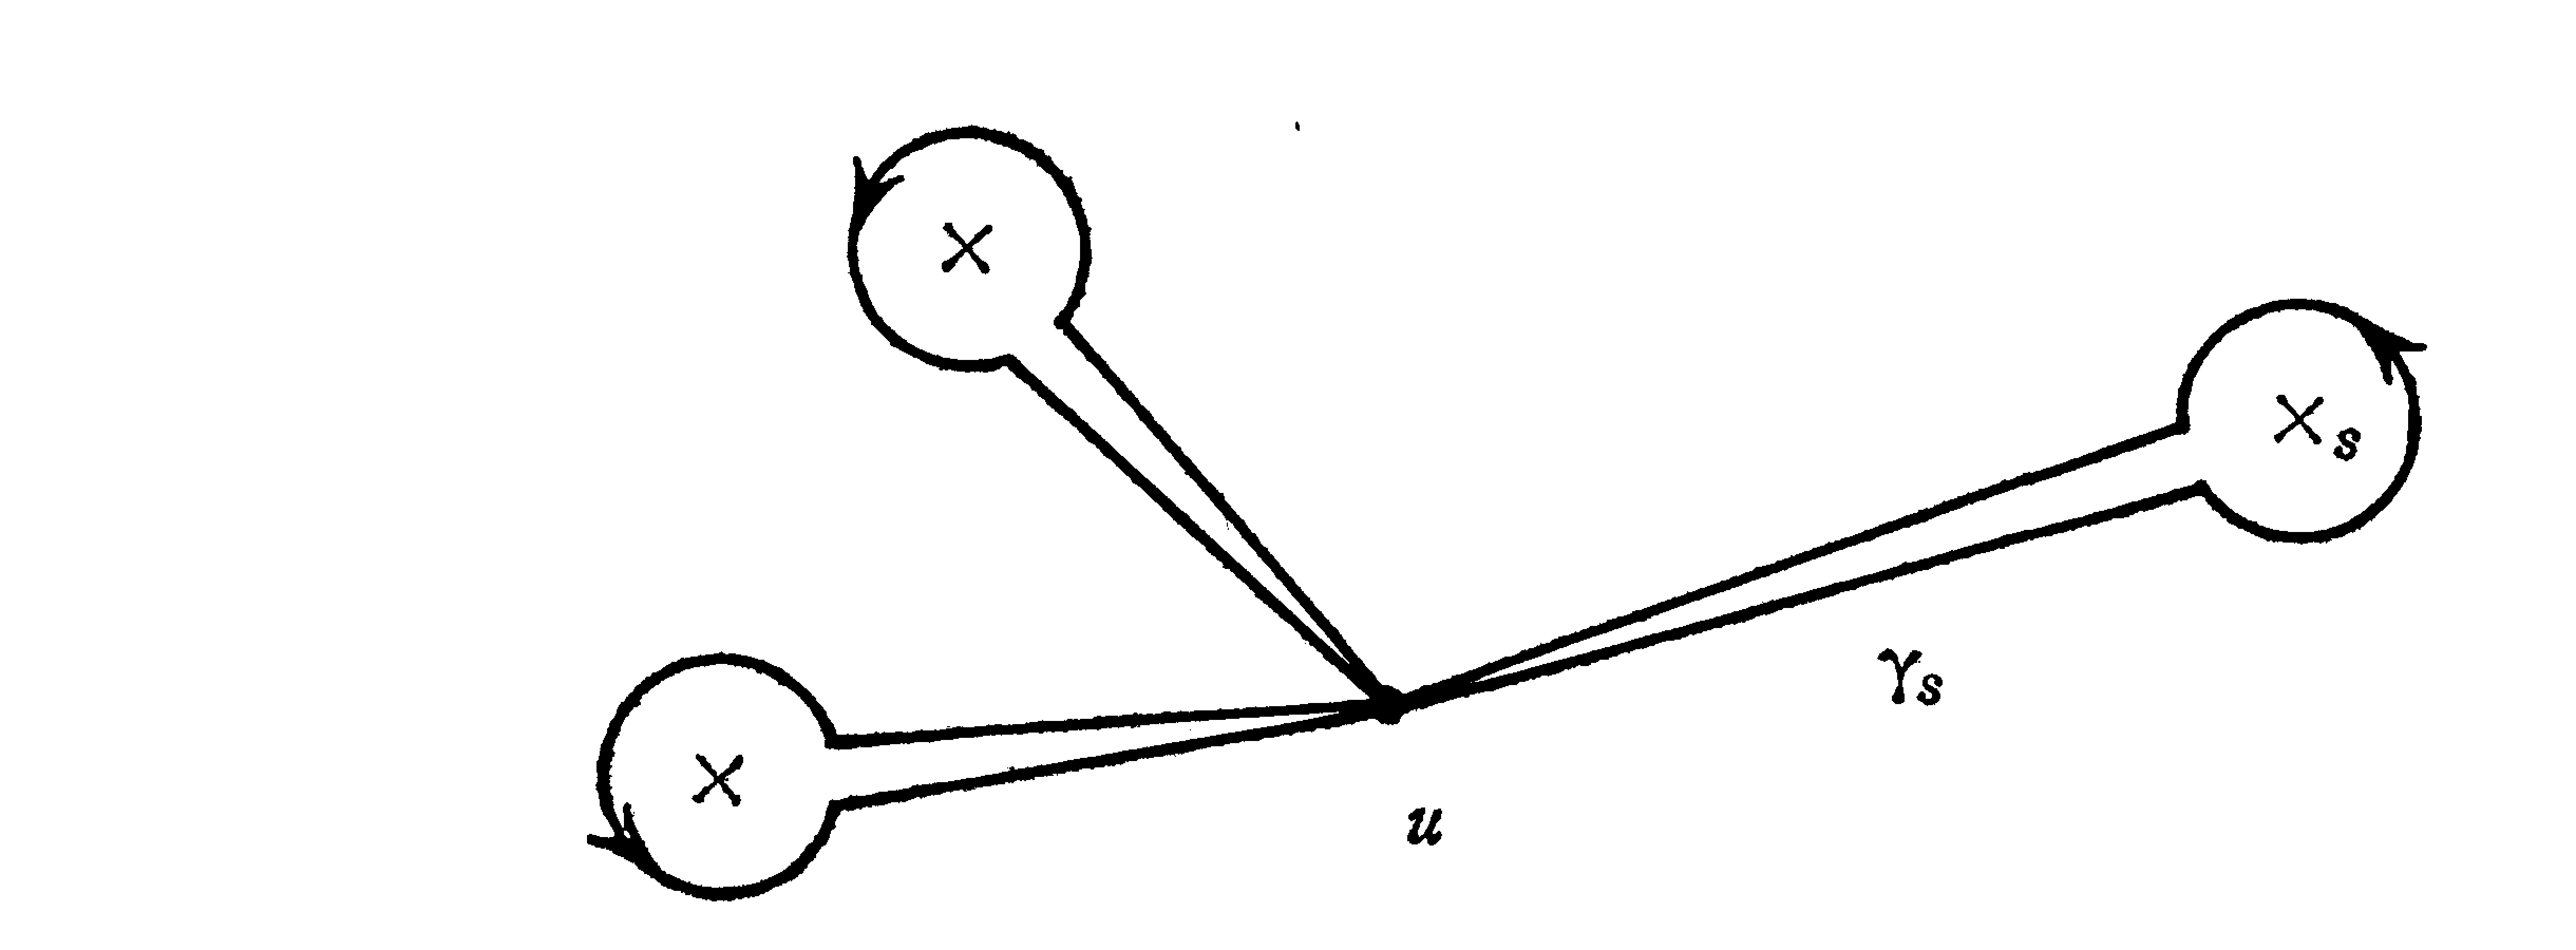
\includegraphics[width=.73\linewidth]{P0019-A01_lacets_presentation.png}\end{center}

\noindent These loops generate the fundamental group \(\pi _{1}(\mathrm{U},u)\). This group acts on \(\mathrm{H}^{i}(\mathrm{X}_{u},\mathbf{Z})\), the fiber at \(u\) of the local system \(\mathrm{R}^{i} f_{*}\mathbf{Z}|\mathrm{U}\). By the local theory (4.1), to each \(s\in \mathrm{S}\) there corresponds a vanishing cycle \(\delta _{s}\in \mathrm{H}^{n}(\mathrm{X}_{u},\mathbf{Z})\); these cycles depend on the choice of the \(\gamma _{s}\). For \(i\ne n\), the action of \(\pi _{1}(\mathrm{U},u)\) on \(\mathrm{H}^{i}(\mathrm{X}_{u},\mathbf{Z})\) is trivial. For \(i=n\), one has\par

\begin{equation*}\begin{gathered}\gamma _{s} x = x \pm  (x,\delta _{s})\delta _{s}.\end{gathered}\tag{5.2.1}\end{equation*}

\noindent Let \(\mathrm{E}\) be the subspace of \(\mathrm{H}^{n}(\mathrm{X}_{u},\mathbf{Q})\) spanned by the \(\delta _{s}\) (the \emph{vanishing part} of the cohomology).\par

\noindent \emph{Proposition} \textbf{(5.3)}. — {\itshape \(\mathrm{E}\) is stable under the action of the monodromy group \(\pi _{1}(\mathrm{U},u)\). The orthogonal complement \(\mathrm{E}^{\perp }\) of \(\mathrm{E}\) (for the intersection form \(\operatorname{Tr}(x\cup y))\) is the subspace of monodromy invariants in \(\mathrm{H}^{n}(\mathrm{X}_{u},\mathbf{Q})\).}\par

\noindent Since the \(\gamma _{s}\) generate the monodromy group, this is clear from (5.2.1).\par

\noindent \emph{Theorem} \textbf{(5.4)}. — {\itshape The vanishing cycles \(\pm \delta _{s}\) (taken up to sign) are conjugate under the action of \(\pi _{1}(\mathrm{U},u)\).}\par

\noindent Let \(\check{\mathrm{X}}\subset \check{\mathbf{P}}\) be the dual variety of \(\mathrm{X}\): it is the set of \(t\in \check{\mathbf{P}}\) such that \(\mathrm{H}_{t}\) is tangent to \(\mathrm{X}\), i.e. such that \(\mathrm{X}_{t}\) is singular, or \(\mathrm{X}\subset \mathrm{H}_{t}\). The variety \(\check{\mathrm{X}}\) is irre-\par

\clearpage

\phantomsection\label{physical-20}\noindent{\footnotesize Authority physical page 20; printed 291}\par\smallskip

\noindent ducible. Let \(\mathrm{Y}\subset \mathrm{X}\times \check{\mathbf{P}}\) be the space of pairs (\(x,t)\) such that \(x\in \mathrm{H}_{t}\). There is a diagram\par

\[\begin{array}{ccc}\mathrm X&\xleftarrow{}&\mathrm Y\\ &&\downarrow\!{g}\\ &&\check{\mathbf P}\end{array}\]

\noindent The fiber of \(g\) at \(t\in \check{\mathbf{P}}\) is the hyperplane section \(\mathrm{X}_{t}=\mathrm{X}\cap \mathrm{H}_{t}\) of \(\mathrm{X}\), and \(g\) is smooth away from the inverse image of \(\check{\mathrm{X}}\).\par

\noindent We recover the situation of (5.1) by replacing \(\check{\mathbf{P}}\) by a line \(\mathrm{D}\subset \check{\mathbf{P}}\) and \(\mathrm{Y}\) by \(g^{- 1}(\mathrm{D})\). Then \(\mathrm{S}=\mathrm{D}\cap \check{\mathrm{X}}\). By a theorem of Lefschetz, for \(\mathrm{D}\) sufficiently general the map\par

\begin{equation*}\begin{gathered}\pi _{1}(\mathrm{D}- \mathrm{S},u) \longrightarrow  \pi _{1}(\check{\mathbf{P}}- \check{\mathrm{X}},u)\end{gathered}\end{equation*}

\noindent is surjective. It is therefore enough to show that the \(\pm \delta _{s}\) are conjugate under \(\pi _{1}(\check{\mathbf{P}}- \check{\mathrm{X}})\).\par

\noindent For \(x\) in the smooth codimension-one locus of \(\check{\mathrm{X}}\), let \(ch\) be a path from \(t\) to \(x\) in \(\check{\mathbf{P}}- \check{\mathrm{X}}\), and let \(\gamma _{x}\) be the loop which follows \(ch\) to a neighborhood of \(\check{\mathrm{X}}\), goes once around \(\check{\mathrm{X}}\), and then returns to \(t\) along \(ch\). The loops \(\gamma _{x}\) (as \(ch\) varies) are conjugate to one another. Since \(\check{\mathrm{X}}\) is irreducible, any two points of its smooth locus can be joined within \(\check{\mathrm{X}}\) by a path which remains in the smooth locus. It follows that the conjugacy class of \(\gamma _{x}\) is independent of \(x\). In particular, the \(\gamma _{s}\) are conjugate to one another. Formula (5.2.1) then shows that the \(\pm \delta _{s}\) are conjugate.\par

\noindent \emph{Corollary} \textbf{(5.5)}. — {\itshape The action of \(\pi _{1}(\mathrm{U},u)\) on \(\mathrm{E}/(\mathrm{E}\cap \mathrm{E}^{\perp })\) is absolutely irreducible.}\par

\noindent Let \(\mathrm{F}\subset \mathrm{E}\otimes \mathbf{C}\) be a subspace stable under monodromy. If \(\mathrm{F}\not\subset (\mathrm{E}\cap \mathrm{E}^{\perp })\otimes \mathbf{C}\), there exist \(x\in \mathrm{F}\) and \(s\in \mathrm{S}\) such that (\(x,\delta _{s})\ne 0\). Then\par

\begin{equation*}\begin{gathered}\gamma _{s} x- x = \pm (x,\delta _{s})\delta _{s} \in  \mathrm{F},\end{gathered}\end{equation*}

\noindent and \(\delta _{s}\in \mathrm{F}\). By (5.4), all the \(\delta _{s}\) then belong to \(\mathrm{F}\), and \(\mathrm{F}=\mathrm{E}\). This proves (5.5).\par

\noindent \textbf{(5.6)} These results transpose as follows to abstract algebraic geometry.\par

\noindent Let \(\mathbf{P}\) be a projective space of dimension >1 over an algebraically closed field \(k\) of characteristic \(p\), and let \(\mathrm{X}\subset \mathbf{P}\) be a connected nonsingular projective variety of dimension \(n+1\). For a linear subspace \(\mathrm{A}\) of \(\mathbf{P}\) of codimension 2, define \(\mathrm{D}\), the pencil (\(\mathrm{H}_{t})_{t\in \mathrm{D}}\), the \(\mathrm{X}_{t}, \widetilde{\mathrm{X}}\), and diagram (5.1.1) as in (5.1). The (\(\mathrm{X}_{t})_{t\in \mathrm{D}}\) are said to form a \emph{Lefschetz pencil} of hyperplane sections if the following conditions hold:\par

\noindent \(\mathrm{A})\) The axis \(\mathrm{A}\) is transverse to \(\mathrm{X}\). The space \(\widetilde{\mathrm{X}}\) is then obtained from \(\mathrm{X}\) by blowing up \(\mathrm{A}\cap \mathrm{X}\), and is smooth.\par

\clearpage

\phantomsection\label{physical-21}\noindent{\footnotesize Authority physical page 21; printed 292}\par\smallskip

\noindent \(\mathrm{B})\) There is a finite subset \(\mathrm{S}\) of \(\mathrm{D}\) and, for each \(s\in \mathrm{S}, a\) point \(x_{s}\in \mathrm{X}_{s}\), such that \(f\) is smooth away from the \(x_{s}\).\par

\noindent \(\mathbf{C}) x_{s}\) is an ordinary quadratic singular point of \(\mathrm{X}_{s}\).\par

\noindent For each \(s\in \mathrm{S}\), the local Lefschetz theory of § 4 applies to the spectrum \(\mathrm{D}_{s}\) of the henselization of the local ring of \(\mathrm{D}\) at \(s\), and to \(\widetilde{\mathrm{X}}_{\mathrm{D}_{s}}=\widetilde{\mathrm{X}}\times _{\mathrm{D}} \mathrm{D}_{s}\).\par

\noindent \textbf{(5.7)} Let \(\mathrm{N}\) be the dimension of \(\mathbf{P}\), let \(r\) be an integer \(\geq 1\), and let \(\iota _{(r)}\) be the embedding of \(\mathbf{P}\) into projective space of dimension \(\binom{\mathrm{N}+r}{\mathrm{N}}- 1\) whose homogeneous coordinates are the monomials of degree \(r\) in the homogeneous coordinates of \(\mathbf{P}\). The hyperplane sections of \(\iota _{(r)}(\mathbf{P})\) are the hypersurfaces of degree \(r\) in \(\mathbf{P}\).\par

\noindent If \(p\ne 0\), it may happen that no pencil of hyperplane sections of \(\mathrm{X}\) is a Lefschetz pencil. Nevertheless, if \(r\geq 2\) and the given projective embedding \(\iota _{1}:\mathrm{X}\hookrightarrow \mathbf{P}\) is replaced by \(\iota _{r}=\iota _{(r)}\circ \iota _{1}\), then, in this new embedding, every sufficiently general pencil is a Lefschetz pencil. In other words, if \(r\geq 2, a\) sufficiently general pencil of hypersurface sections of degree \(r\) of \(\mathrm{X}\) is always a Lefschetz pencil.\par

\noindent \textbf{(5.8)} In the remainder of this discussion we study a Lefschetz pencil of hyperplane sections of \(\mathrm{X}\), \emph{excluding the case \(p=2\) with \(n\) even}. The case in which \(n\) is odd would suffice for what follows. Put \(\mathrm{U}=\mathrm{D}- \mathrm{S}\). Let \(u\in \mathrm{U}\) and let \(\ell \) be a prime \(\ne p\). The local results of § 4 show that \(\mathrm{R}^{n} f_{*}\mathbf{Q}_{\ell }\) is \emph{tamely} ramified at each \(s\in \mathrm{S}\). The tame fundamental group of \(\mathrm{U}\) is a quotient of the profinite completion of the analogous transcendental fundamental group (lifting tame coverings to characteristic 0, and the Riemann existence theorem). The algebraic situation is therefore entirely analogous to the transcendental one, and the Lefschetz results transpose by standard arguments. In the proof of (5.4), the Lefschetz theorem on fundamental groups becomes Bertini's theorem, and one must invoke Abhyankar's lemma to control the ramification of \(\mathrm{R}^{i} g_{*}\mathbf{Q}_{\ell }\) along the smooth codimension-one locus of \(\check{\mathrm{X}}\).\par

\noindent The results are as follows.\par

\noindent a) \emph{If the vanishing cycles are nonzero:}\par

\noindent 1) For \(i\ne n\), the sheaf \(\mathrm{R}^{i} f_{*}\mathbf{Q}_{\ell }\) on \(\mathrm{D}\) is constant.\par

\noindent 2) Let \(j\) be the inclusion of \(\mathrm{U}\) in \(\mathrm{D}\). Then\par

\begin{equation*}\begin{gathered}\mathrm{R}^{n} f_{*}\mathbf{Q}_{\ell } = j_{*}j^{*}\mathrm{R}^{n} f_{*}\mathbf{Q}_{\ell }.\end{gathered}\end{equation*}

\noindent 3) Let \(\mathrm{E}\subset \mathrm{H}^{n}(\mathrm{X}_{u},\mathbf{Q}_{\ell })\) be the subspace of cohomology spanned by the vanishing cycles. This subspace is stable under \(\pi _{1}(\mathrm{U},u)\), and\par

\begin{equation*}\begin{gathered}\mathrm{E}^{\perp } = \mathrm{H}^{n}(\mathrm{X}_{u},\mathbf{Q}_{\ell })^{\pi _{1}(\mathrm{U},u)}.\end{gathered}\end{equation*}

\noindent The representation of \(\pi _{1}(\mathrm{U},u)\) on \(\mathrm{E}/(\mathrm{E}\cap \mathrm{E}^{\perp })\) is absolutely irreducible, and the image of \(\pi _{1}\) in \(\operatorname{GL}(\mathrm{E}/(\mathrm{E}\cap \mathrm{E}^{\perp }))\) is generated (topologically) by the maps \(x\longmapsto x\pm (x,\delta _{s})\delta _{s} (s\in \mathrm{S})\), with the sign \(\pm \) determined as in (4.1).\par

\clearpage

\phantomsection\label{physical-22}\noindent{\footnotesize Authority physical page 22; printed 293}\par\smallskip

\noindent \(b)\) \emph{If the vanishing cycles are zero:} (This is an exceptional case. Since (\(\delta ,\delta )=\pm 2\) for \(n\) even, it can occur only when \(n\) is odd: \(n=2m+1\). Note that if one vanishing cycle is zero, then all are zero, since they are conjugate.)\par

\noindent 1) For \(i\ne n+1\), the sheaf \(\mathrm{R}^{i} f_{*}\mathbf{Q}_{\ell }\) is constant.\par

\noindent 2) There is an exact sequence\par

\begin{equation*}\begin{gathered}0 \longrightarrow  \bigoplus\limits_{s\in \mathrm{S}} \mathbf{Q}_{\ell }(m- n)_{s} \longrightarrow  \mathrm{R}^{n+1}f_{*}\mathbf{Q}_{\ell } \longrightarrow  \mathcal{F}  \longrightarrow  0\end{gathered}\end{equation*}

\noindent with \(\mathcal{F} \) constant.\par

\noindent \(3) \mathrm{E}=0\).\par

\noindent \textbf{(5.9)} The subspace \(\mathrm{E}\cap \mathrm{E}^{\perp }\) of \(\mathrm{E}\) is the kernel of the restriction to \(\mathrm{E}\) of the intersection form \(\operatorname{Tr}(x\cup y)\). This form therefore induces a nondegenerate bilinear form\par

\begin{equation*}\begin{gathered}\psi  : \mathrm{E}/(\mathrm{E}\cap \mathrm{E}^{\perp })\otimes \mathrm{E}/(\mathrm{E}\cap \mathrm{E}^{\perp }) \longrightarrow  \mathbf{Q}_{\ell }(- n),\end{gathered}\end{equation*}

\noindent alternating for \(n\) odd and symmetric for \(n\) even. This form is preserved by monodromy; for \(n\) odd, the monodromy representation therefore induces\par

\begin{equation*}\begin{gathered}\rho  : \pi _{1}(\mathrm{U},u) \longrightarrow  \operatorname{Sp}(\mathrm{E}/(\mathrm{E}\cap \mathrm{E}^{\perp }),\psi ).\end{gathered}\end{equation*}

\noindent \emph{Theorem} \textbf{(5.10)} (Kajdan-Margulis). — {\itshape The image of \(\rho \) is open.}\par

\noindent The image of \(\rho \) is a compact, hence \(\ell \)-adic analytic, subgroup of \(\operatorname{Sp}(\mathrm{E}/(\mathrm{E}\cap \mathrm{E}^{\perp }),\psi )\). It is enough to show that its Lie algebra \(\mathfrak{L} \) is equal to \(\mathfrak{sp}(\mathrm{E}/(\mathrm{E}\cap \mathrm{E}^{\perp }),\psi )\). The transcendental analogue of this Lie algebra is the Lie algebra of the Zariski closure of the monodromy group.\par

\noindent It follows from (5.8) that \(\mathfrak{L} \) is generated by the square-zero transformations\par

\begin{equation*}\begin{gathered}\mathrm{N}_{s} : x \longmapsto  (x,\delta _{s})\delta _{s}    (s\in \mathrm{S})\end{gathered}\end{equation*}

\noindent and that \(\mathrm{E}/(\mathrm{E}\cap \mathrm{E}^{\perp })\) is an absolutely irreducible representation of \(\mathfrak{L} \). The theorem follows from the next lemma.\par

\noindent \emph{Lemma} \textbf{(5.11)}. — {\itshape Let \(\mathrm{V}\) be a finite-dimensional vector space over a field \(k\) of characteristic 0, let \(\psi \) be a nondegenerate alternating form, and let \(\mathfrak{L} \) be a Lie subalgebra of \(\mathfrak{sp}(\mathrm{V},\psi )\). Suppose that:}\par

\noindent {\itshape \textup{(i)} \(\mathrm{V}\) is a simple representation of \(\mathfrak{L} \).}\par

\noindent {\itshape \textup{(ii)} \(\mathfrak{L} \) is generated by a family of endomorphisms of \(\mathrm{V}\) of the form \(x\longmapsto \psi (x,\delta )\delta \).}\par

\noindent {\itshape Then \(\mathfrak{L} =\mathfrak{sp}(\mathrm{V},\psi )\).}\par

\noindent We may and shall suppose that \(\mathrm{V}\), and hence \(\mathfrak{L} \), is nonzero. Let \(\mathrm{W}\subset \mathrm{V}\) be the set of \(\delta \in \mathrm{V}\) such that \(\mathrm{N}(\delta ):x\longmapsto \psi (x,\delta )\delta \) belongs to \(\mathfrak{L} \).\par

\noindent a) \(\mathrm{W}\) is stable under homotheties (since \(\mathfrak{L} \) is a vector subspace of \(\mathfrak{gl}(\mathrm{V}))\).\par

\noindent \(b)\) If \(\delta \in \mathrm{W}, \operatorname{exp}(\lambda \mathrm{N}(\delta ))\) is an automorphism of (\(\mathrm{V},\psi ,\mathfrak{L} )\), and therefore carries \(\mathrm{W}\) into itself. If \(\delta ',\delta ''\in \mathrm{W}\), then \(\operatorname{exp}(\lambda \mathrm{N}(\delta '))\cdot \delta ''=\delta ''+\lambda \psi (\delta '',\delta ')\delta '\in \mathrm{W}\); if \(\psi (\delta ',\delta '')\ne 0\), the linear subspace spanned by \(\delta '\) and \(\delta ''\) lies in \(\mathrm{W}\).\par

\clearpage

\phantomsection\label{physical-23}\noindent{\footnotesize Authority physical page 23; printed 294}\par\smallskip

\noindent \(c)\) It follows that \(\mathrm{W}\) is the union of its maximal linear subspaces \(\mathrm{W}_{\alpha }\), and that these are pairwise orthogonal. Each \(\mathrm{W}_{\alpha }\) is therefore stable under the \(\mathrm{N}(\delta ) (\delta \in \mathrm{W})\), hence stable under \(\mathfrak{L} \). By hypothesis (\(i), \mathrm{W}_{\alpha }=\mathrm{V}\), and \(\mathfrak{L} \) contains every \(\mathrm{N}(\delta )\) for \(\delta \in \mathrm{V}\). We conclude by observing that the Lie algebra \(\mathfrak{sp}(\mathrm{V},\psi )\) is generated by the \(\mathrm{N}(\delta ) (\delta \in \mathrm{V})\).\par

\noindent \emph{Remark} \textbf{(5.12)} (not used below). — It is now easy to prove (1.6) for a hypersurface of odd dimension \(n\) in \(\mathbf{P}^{n+1}_{\mathbf{F}_{q}}\).\par

\noindent Let \(\mathrm{X}_{0}\) be such a hypersurface, and let \(\overline{\mathrm{X}}_{0}\) be the hypersurface over \(\overline{\mathbf{F}}_{q}\) obtained from it by extension of scalars. One has\par

\begin{equation*}\begin{gathered}\mathrm{H}^{2i}(\overline{\mathrm{X}}_{0},\mathbf{Q}_{\ell })=\mathbf{Q}_{\ell }(- i)    (0\leq i\leq n);\end{gathered}\end{equation*}

\noindent \(\mathrm{H}^{2i}(\overline{\mathrm{X}}_{0},\mathbf{Q}_{\ell }(i))\) is generated by the \(i\)-th cup power of \(\eta \), the cohomology class \(c_{1}(\mathcal{O}(1))\) of a hyperplane section. Hence\par

\begin{equation*}\begin{gathered}\mathrm{Z}(\mathrm{X}_{0},t)=\operatorname{det}(1- \mathrm{F}^{*}t,\mathrm{H}^{n}(\overline{\mathrm{X}}_{0},\mathbf{Q}_{\ell })) / \prod _{i=0}^{n}(1- q^{i} t),\end{gathered}\end{equation*}

\noindent and \(\operatorname{det}(1- \mathrm{F}^{*}t,\mathrm{H}^{n}(\overline{\mathrm{X}}_{0},\mathbf{Q}_{\ell }))\) is a polynomial with integer coefficients independent of \(\ell \).\par

\noindent Let \(\mathrm{X}_{0}\) vary in a Lefschetz pencil of hypersurfaces defined over \(\mathbf{F}_{q}\) (cf. (5.7) for \(\mathrm{X}=\mathbf{P}^{n+1}\); the existence of such a pencil is not clear; to complete the argument sketched here one would have to use the arguments to be given in (7.1)). One checks that here \(\mathrm{E}\) coincides with the whole \(\mathrm{H}^{n}\), and (3.2) gives the Weil conjecture for every hypersurface in the pencil, in particular for \(\mathrm{X}_{0}\).\par

\noindent \textbf{(5.13)} \emph{Bibliographical indications for §§ 4 and 5.}\par

\noindent \(\mathrm{A})\) Lefschetz's results (4.1) and (5.1) through (5.5) are contained in his book [2]. For the local theory (4.1), it may be more convenient to consult SGA 7, XIV (3.2).\par

\noindent \(\mathrm{B})\) The results of § 4 are proved in Exposés XIII, XIV, and XV of SGA 7.\par

\noindent C) (5.7) is proved in SGA 7, XVII.\par

\noindent D) (5.8) is proved in SGA 7, XVIII. The irreducibility theorem is proved there for \(\mathrm{E}\), but only under the hypothesis \(\mathrm{E}\cap \mathrm{E}^{\perp }=\{0\}\). The proof in the general case, for \(\mathrm{E}/(\mathrm{E}\cap \mathrm{E}^{\perp })\), is the same.\par

\section*{6. A rationality theorem.}

\noindent \textbf{(6.1)} Let \(\mathbf{P}_{0}\) be a projective space of dimension \(\geq 1\) over \(\mathbf{F}_{q}\), let \(\mathrm{X}_{0}\subset \mathbf{P}_{0}\) be a nonsingular projective variety, let \(\mathrm{A}_{0}\subset \mathbf{P}_{0}\) be a linear subspace of codimension two, let \(\mathrm{D}_{0}\subset \check{\mathbf{P}}_{0}\) be the dual line, let \(\overline{\mathbf{F}}_{q}\) be an algebraic closure of \(\mathbf{F}_{q}\), and let \(\mathbf{P}, \mathrm{X}, \mathrm{A}, \mathrm{D}\) over \(\overline{\mathbf{F}}_{q}\) be obtained from \(\mathbf{P}_{0}, \mathrm{X}_{0}\),\par

\clearpage

\phantomsection\label{physical-24}\noindent{\footnotesize Authority physical page 24; printed 295}\par\smallskip

\noindent \(\mathrm{A}_{0}, \mathrm{D}_{0}\) by extension of scalars. Diagram (5.1.1) of (5.6) comes from an analogous diagram over \(\mathbf{F}_{q}\):\par

\[\begin{array}{ccc}\mathrm X_0&\xleftarrow{\pi_0}&\widetilde{\mathrm X}_0\\ &&\downarrow\!{f_0}\\ &&\mathrm D_0\end{array}\tag{6.1.1}\]

\noindent Suppose that \(\mathrm{X}\) is connected of \emph{even} dimension \(n+1=2m+2\), and that the pencil (\(\mathrm{X}_{t})_{t\in \mathrm{D}}\) of hyperplane sections of \(\mathrm{X}\) defined by \(\mathrm{D}\) is a \emph{Lefschetz pencil}. The set \(\mathrm{S}\) of \(t\in \mathrm{D}\) for which \(\mathrm{X}_{t}\) is singular is defined over \(\mathbf{F}_{q}\), i.e. comes from \(\mathrm{S}_{0}\subset \mathrm{D}_{0}\). Put \(\mathrm{U}_{0}=\mathrm{D}_{0}- \mathrm{S}_{0}\) and \(\mathrm{U}=\mathrm{D}- \mathrm{S}\).\par

\noindent Let \(u\in \mathrm{U}\). The vanishing part \(\mathrm{E}\subset \mathrm{H}^{n}(\mathrm{X}_{u},\mathbf{Q}_{\ell })\) of the cohomology is stable under \(\pi _{1}(\mathrm{U},u)\), and therefore defines on \(\mathrm{U}\) a local subsystem \(\mathcal{E} \) of \(\mathrm{R}^{n} f_{*}\mathbf{Q}_{\ell }\). The latter is defined over \(\mathbf{F}_{q}: \mathrm{R}^{i} f_{*}\mathbf{Q}_{\ell }\) is the inverse image of the \(\mathbf{Q}_{\ell }\)-sheaf \(\mathrm{R}^{i} f_{0*}\mathbf{Q}_{\ell }\) on \(\mathrm{D}_{0}\), and, on \(\mathrm{U}, \mathcal{E} \) is the inverse image of a local subsystem\par

\begin{equation*}\begin{gathered}\mathcal{E} _{0} \subset  \mathrm{R}^{n} f_{0*}\mathbf{Q}_{\ell }.\end{gathered}\end{equation*}

\noindent The cup product is an alternating form\par

\begin{equation*}\begin{gathered}\psi  : \mathrm{R}^{n} f_{0*}\mathbf{Q}_{\ell }\otimes \mathrm{R}^{n} f_{0*}\mathbf{Q}_{\ell } \longrightarrow  \mathbf{Q}_{\ell }(- n).\end{gathered}\end{equation*}

\noindent Let \(\mathcal{E} _{0}^{\perp }\) denote the orthogonal complement of \(\mathcal{E} _{0}\) with respect to \(\psi \). On \(\mathrm{R}^{n} f_{0*}\mathbf{Q}_{\ell }|\mathrm{U}_{0}\), one sees that \(\psi \) induces a perfect duality\par

\begin{equation*}\begin{gathered}\psi  : \mathcal{E} _{0}/(\mathcal{E} _{0}\cap \mathcal{E} _{0}^{\perp })\otimes \mathcal{E} _{0}/(\mathcal{E} _{0}\cap \mathcal{E} _{0}^{\perp }) \longrightarrow  \mathbf{Q}_{\ell }(- n).\end{gathered}\end{equation*}

\noindent \emph{Theorem} \textbf{(6.2)}. — {\itshape For every \(x\in |\mathrm{U}_{0}|\), the polynomial \(\operatorname{det}(1- \mathrm{F}_{x}^{*}t,\mathcal{E} _{0}/(\mathcal{E} _{0}\cap \mathcal{E} _{0}^{\perp }))\) has rational coefficients.}\par

\noindent \emph{Corollary} \textbf{(6.3)}. — {\itshape Let \(j_{0}\) be the inclusion of \(\mathrm{U}_{0}\) in \(\mathrm{D}_{0}\), and \(j\) that of \(\mathrm{U}\) in \(\mathrm{D}\). The eigenvalues of \(\mathrm{F}^{*}\) acting on \(\mathrm{H}^{1}(\mathrm{D},j_{*}\mathcal{E} /(\mathcal{E} \cap \mathcal{E} ^{\perp }))\) are algebraic numbers all of whose complex conjugates \(\alpha \) satisfy}\par

\begin{equation*}\begin{gathered}q^{\frac{n+1}{2}- \frac{1}{2}} \leq  |\alpha | \leq  q^{\frac{n+1}{2}+\frac{1}{2}}.\end{gathered}\end{equation*}

\noindent Indeed, by (5.10) and (6.2), the hypotheses of (3.2) are satisfied by (\(\mathrm{U}_{0},\mathcal{E} _{0}/(\mathcal{E} _{0}\cap \mathcal{E} _{0}^{\perp }),\psi )\), with \(\beta =n\), and one applies (3.9).\par

\noindent \emph{Lemma} \textbf{(6.4)}. — {\itshape Let \(\mathcal{G} _{0}\) be a twisted constant \(\mathbf{Q}_{\ell }\)-sheaf on \(\mathrm{U}_{0}\) whose inverse image \(\mathcal{G} \) on \(\mathrm{U}\) is a constant sheaf. Then there exist \(\ell \)-adic units \(\alpha _{i}\) in \(\overline{\mathbf{Q}}_{\ell }\) such that, for every \(x\in |\mathrm{U}_{0}|\),}\par

\begin{equation*}\begin{gathered}\operatorname{det}(1- \mathrm{F}_{x}^{*}t,\mathcal{G} _{0})=\prod _{i}(1- \alpha _{i}^{\operatorname{deg}(x)}t).\end{gathered}\end{equation*}

\clearpage

\phantomsection\label{physical-25}\noindent{\footnotesize Authority physical page 25; printed 296}\par\smallskip

\noindent This lemma says that \(\mathcal{G} _{0}\) is the inverse image of a sheaf on \(\operatorname{Spec}(\mathbf{F}_{q})\), namely its direct image on \(\operatorname{Spec}(\mathbf{F}_{q})\). The latter identifies with an \(\ell \)-adic representation \(\mathrm{G}_{0}\) of \(\operatorname{Gal}(\overline{\mathbf{F}}_{q}/\mathbf{F}_{q})\), and we take\par

\begin{equation*}\begin{gathered}\operatorname{det}(1- \mathrm{F}t,\mathrm{G}_{0})=\prod _{i}(1- \alpha _{i} t).\end{gathered}\end{equation*}

\noindent Lemma (6.4) applies to \(\mathrm{R}^{i} f_{0*}\mathbf{Q}_{\ell } (i\ne n)\), to \(\mathrm{R}^{n} f_{0*}\mathbf{Q}_{\ell }/\mathcal{E} _{0}\), and to \(\mathcal{E} _{0}\cap \mathcal{E} _{0}^{\perp }\).\par

\noindent For \(x\in |\mathrm{U}_{0}|\), the fiber \(\mathrm{X}_{x}=f_{0}^{- 1}(x)\) is a variety over the finite field \(k(x)\). If \(\overline{x}\) is a point of \(\mathrm{U}\) above \(x, \mathrm{X}_{\overline{x}}\) is obtained from \(\mathrm{X}_{x}\) by extension of scalars from \(k(x)\) to its algebraic closure \(k(\overline{x})=\overline{\mathbf{F}}_{q}\), and \(\mathrm{H}^{i}(\mathrm{X}_{\overline{x}},\mathbf{Q}_{\ell })\) is the fiber of \(\mathrm{R}^{i} f_{*}\mathbf{Q}_{\ell }\) at \(\overline{x}\). Formula (1.5.4) for the variety \(\mathrm{X}_{x}\) over \(k(x)\) therefore reads\par

\begin{equation*}\begin{gathered}\mathrm{Z}(\mathrm{X}_{x},t)=\prod _{i} \operatorname{det}(1- \mathrm{F}_{x}^{*}t,\mathrm{R}^{i} f_{0*}\mathbf{Q}_{\ell })^{(- 1)^{i+1}},\end{gathered}\end{equation*}

\noindent and \(\mathrm{Z}(\mathrm{X}_{x},t)\) is the product of\par

\begin{equation*}\begin{gathered}\mathrm{Z}^{f}=\operatorname{det}(1- \mathrm{F}_{x}^{*}t,\mathrm{R}^{n} f_{0*}\mathbf{Q}_{\ell }/\mathcal{E} _{0})\cdot \operatorname{det}(1- \mathrm{F}_{x}^{*}t,\mathcal{E} _{0}\cap \mathcal{E} _{0}^{\perp }) \\ \cdot \prod _{i\ne n} \operatorname{det}(1- \mathrm{F}_{x}^{*}t,\mathrm{R}^{i} f_{0*}\mathbf{Q}_{\ell })^{(- 1)^{i+1}}\end{gathered}\end{equation*}

\noindent and\par

\begin{equation*}\begin{gathered}\mathrm{Z}^{m}=\operatorname{det}(1- \mathrm{F}_{x}^{*}t,\mathcal{E} _{0}/(\mathcal{E} _{0}\cap \mathcal{E} _{0}^{\perp })).\end{gathered}\end{equation*}

\noindent Put \(\mathcal{F} _{0}=\mathcal{E} _{0}/(\mathcal{E} _{0}\cap \mathcal{E} _{0}^{\perp }), \mathcal{F} =\mathcal{E} /(\mathcal{E} \cap \mathcal{E} ^{\perp })\), and apply (6.4) to the factors of \(\mathrm{Z}^{f}\). We find that there exist \(\ell \)-adic units \(\alpha _{i} (1\leq i\leq \mathrm{N})\) and \(\beta _{j} (1\leq j\leq \mathrm{M})\) in \(\overline{\mathbf{Q}}_{\ell }\) such that for every \(x\in |\mathrm{U}_{0}|\)\par

\[\mathrm{Z}(\mathrm{X}_{x},t)=\frac{\prod\limits _{i}(1- \alpha _{i}^{\operatorname{deg}(x)}t)}{\prod\limits _{j}(1- \beta _{j}^{\operatorname{deg}(x)}t)}\cdot \operatorname{det}(1- \mathrm{F}_{x}^{*}t,\mathcal{F} _{0}),\]

\noindent and in particular the right-hand side belongs to \(\mathbf{Q}(t)\). If an \(\alpha _{i}\) coincides with a \(\beta _{j}\), it is permissible to delete simultaneously that \(\alpha _{i}\) from the list of the \(\alpha 's\) and that \(\beta _{j}\) from the list of the \(\beta 's\). We may therefore suppose, and shall suppose, that \(\alpha _{i}\ne \beta _{j}\) for every \(i\) and \(j\).\par

\noindent \textbf{(6.5)} It is enough to prove that the polynomials \(\prod _{i}(1- \alpha _{i} t)\) and \(\prod _{j}(1- \beta _{j} t)\) have rational coefficients, i.e. that the family of the \(\alpha _{i}\) (respectively, the family of the \(\beta _{j})\) is defined over \(\mathbf{Q}\). We shall deduce this from the following propositions.\par

\noindent \emph{Proposition} \textbf{(6.6)}. — {\itshape Let (\(\gamma _{i}) (1\leq i\leq \mathrm{P})\) and (\(\delta _{j}) (1\leq j\leq \mathrm{Q})\) be two families of \(\ell \)-adic units in \(\overline{\mathbf{Q}}_{\ell }\). Suppose that \(\gamma _{i}\ne \delta _{j}\). If \(\mathrm{K}\) is a sufficiently large finite set of integers different from 1, and \(\mathrm{L}\) is a sufficiently large subset of |\(\mathrm{U}_{0}|\) of density 0, then, whenever \(x\in |\mathrm{U}_{0}|\) satisfies \(k\nmid \operatorname{deg}(x)\) (for every \(k\in \mathrm{K})\) and \(x\notin \mathrm{L}\), the denominator of}\par

\begin{equation*}\begin{gathered}\operatorname{det}(1- \mathrm{F}_{x}^{*}t,\mathcal{F} _{0})\cdot \prod _{i}(1- \gamma _{i}^{\operatorname{deg}(x)}t) / \prod _{j}(1- \delta _{j}^{\operatorname{deg}(x)}t),\end{gathered}\tag{6.6.1}\end{equation*}

\noindent {\itshape when written in lowest terms, is \(\prod _{j}(1- \delta _{j}^{\operatorname{deg}(x)}t)\).}\par

\noindent The proof will be given in (6.10-13). By (6.7) below, (6.6) gives\par

\clearpage

\phantomsection\label{physical-26}\noindent{\footnotesize Authority physical page 26; printed 297}\par\smallskip

\noindent an intrinsic description of the family of the \(\delta _{j}\) in terms of the family of rational functions (6.6.1), for \(x\in |\mathrm{U}_{0}|\).\par

\noindent \emph{Lemma} \textbf{(6.7)}. — {\itshape Let \(\mathrm{K}\) be a finite set of integers different from 1, and let (\(\delta _{j}) (1\leq j\leq \mathrm{Q})\) and (\(\varepsilon _{j}) (1\leq j\leq \mathrm{Q})\) be two families of elements of a field. If, for every sufficiently large \(n\) divisible by none of the \(k\in \mathrm{K}\), the family of the \(\delta _{j}^{n}\) coincides with that of the \(\varepsilon _{j}^{n}\) (up to order), then the family of the \(\delta _{j}\) coincides with that of the \(\varepsilon _{j}\) (up to order).}\par

\noindent We argue by induction on \(\mathrm{Q}\). The set of integers \(n\) such that \(\delta _{\mathrm{Q}}^{n}=\varepsilon _{j}^{n}\) is an ideal (\(n_{j})\). Let us prove that there is a \(j_{0}\) such that \(\delta _{\mathrm{Q}}=\varepsilon _{j_{0}}\). Otherwise the \(n_{j}\) would all be different from 1, and there would be arbitrarily large integers \(n\) divisible by none of the \(n_{j}\) and by none of the \(k\in \mathrm{K}\). We would then have \(\delta _{\mathrm{Q}}^{n}\ne \varepsilon _{j}^{n}\), contradicting the hypothesis. Thus there is a \(j_{0}\) such that \(\delta _{\mathrm{Q}}=\varepsilon _{j_{0}}\). The conclusion follows by applying the induction hypothesis to the families (\(\delta _{j}) (j\ne \mathrm{Q})\) and (\(\varepsilon _{j}) (j\ne j_{0})\).\par

\noindent \emph{Proposition} \textbf{(6.8)}. — {\itshape Let (\(\gamma _{i}) (1\leq i\leq \mathrm{P})\) and (\(\delta _{j}) (1\leq j\leq \mathrm{Q})\) be two families of \(p\)-adic units in \(\overline{\mathbf{Q}}_{\ell }\), and put \(\mathrm{R}(t)=\prod _{i}(1- \gamma _{i} t)\) and \(\mathrm{S}(t)=\prod _{j}(1- \delta _{j} t)\). Suppose that for every \(x\in |\mathrm{U}_{0}|\),}\par

\begin{equation*}\begin{gathered}\prod _{i}(1- \delta _{i}^{\operatorname{deg}(x)}t)\text{ divides } \\ \prod _{i}(1- \gamma _{i}^{\operatorname{deg}(x)}t)\cdot \operatorname{det}(1- \mathrm{F}_{x}^{*}t,\mathcal{F} _{0}).\end{gathered}\end{equation*}

\noindent {\itshape Then \(\mathrm{S}(t)\) divides \(\mathrm{R}(t)\).}\par

\noindent Remove from the families (\(\gamma _{i})\) and (\(\delta _{j})\) pairs of common elements until the hypothesis of (6.6) is satisfied. Apply (6.6). By hypothesis, the rational functions (6.6.1) are polynomials. No \(\delta \) therefore remains, which means that \(\mathrm{S}(t)\) divides \(\mathrm{R}(t)\).\par

\noindent This proposition gives an intrinsic characterization of \(\mathrm{R}(t)\) in terms of the family of polynomials\par

\begin{equation*}\begin{gathered}\prod _{i}(1- \gamma _{i}^{\operatorname{deg}(x)}t)\cdot \operatorname{det}(1- \mathrm{F}_{x}^{*}t,\mathcal{F} _{0}).\end{gathered}\end{equation*}

\noindent It is the least common multiple of the polynomials \(\mathrm{S}(t)=\prod _{j}(1- \delta _{j} t)\) satisfying the hypothesis of (6.8).\par

\noindent \textbf{(6.9)} Let us prove (6.5), and hence (6.2), modulo (6.6). In (6.6), take (\(\gamma _{i})=(\alpha _{i})\) and (\(\delta _{j})=(\beta _{j})\). We obtain an intrinsic characterization of the family of the \(\beta _{j}\) in terms of the family of rational functions \(\mathrm{Z}(\mathrm{X}_{x},t) (x\in |\mathrm{U}_{0}|)\). Since these belong to \(\mathbf{Q}(t)\), the family of the \(\beta _{j}\) is defined over \(\mathbf{Q}\).\par

\noindent The polynomials \(\prod _{i}(1- \alpha _{i}^{\operatorname{deg}(x)}t)\cdot \operatorname{det}(1- \mathrm{F}_{x}^{*}t,\mathcal{F} _{0})\) therefore belong to \(\mathbf{Q}[t]\). Proposition (6.8) gives an intrinsic description of the family of the \(\alpha _{i}\) in terms of this family of polynomials. The family of the \(\alpha _{i}\) is therefore defined over \(\mathbf{Q}\).\par

\noindent \textbf{(6.10)} \emph{Preliminaries}. — Let \(u\in \mathrm{U}\), and let \(\mathcal{F} _{u}\) be the fiber of \(\mathcal{F} \) at \(u\). The arithmetic fundamental group \(\pi _{1}(\mathrm{U}_{0},u)\), an extension of \(\widehat{\mathbf{Z}}=\operatorname{Gal}(\overline{\mathbf{F}}_{q}/\mathbf{F}_{q})\) (generator: \(\varphi )\) by the geometric fundamental group \(\pi _{1}(\mathrm{U},u)\), acts on \(\mathcal{F} _{u}\) by symplectic similitudes:\par

\begin{equation*}\begin{gathered}\rho  : \pi _{1}(\mathrm{U}_{0},u) \longrightarrow  \operatorname{CSp}(\mathcal{F} _{u},\psi ).\end{gathered}\end{equation*}

\clearpage

\phantomsection\label{physical-27}\noindent{\footnotesize Authority physical page 27; printed 298}\par\smallskip

\noindent We denote by \(\mu (g)\) the multiplier of a symplectic similitude \(g\). Let\par

\begin{equation*}\begin{gathered}\mathrm{H}\subset \widehat{\mathbf{Z}}\times \operatorname{CSp}(\mathcal{F} _{u},\psi )\end{gathered}\end{equation*}

\noindent be the subgroup defined by the equation\par

\begin{equation*}\begin{gathered}q^{- n}=\mu (g)\end{gathered}\end{equation*}

\noindent (\(q\) being an \(\ell \)-adic unit, \(q^{n}\in \mathbf{Q}_{\ell }^{*}\) is defined for every \(n\in \widehat{\mathbf{Z}})\). The fact that \(\psi \) takes values in \(\mathbf{Q}_{\ell }(- n)\) is expressed by saying that the map from \(\pi _{1}\) to \(\widehat{\mathbf{Z}}\times \operatorname{CSp}\), whose components are the canonical projection onto \(\widehat{\mathbf{Z}}\) and \(\rho \), factors through\par

\begin{equation*}\begin{gathered}\rho _{1} : \pi _{1}(\mathrm{U}_{0},u) \longrightarrow  \mathrm{H}.\end{gathered}\end{equation*}

\noindent \emph{Lemma} \textbf{(6.11)}. — {\itshape The image \(\mathrm{H}_{1}\) of \(\rho _{1}\) is open in \(\mathrm{H}\).}\par

\noindent Indeed, \(\pi _{1}(\mathrm{U}_{0},u)\) maps onto \(\widehat{\mathbf{Z}}\), and the image of \(\pi _{1}(\mathrm{U},u)=\operatorname{Ker}(\pi _{1}(\mathrm{U}_{0},u)\longrightarrow \widehat{\mathbf{Z}})\) in \(\operatorname{Sp}(\mathcal{F} _{u},\psi )=\operatorname{Ker}(\mathrm{H}\longrightarrow \widehat{\mathbf{Z}})\) is open by (5.10).\par

\noindent \emph{Lemma} \textbf{(6.12)}. — {\itshape For an \(\ell \)-adic unit \(\delta \in \overline{\mathbf{Q}}_{\ell }\), the set \(\mathrm{Z}\) of (\(n,g)\in \mathrm{H}_{1}\) such that \(\delta ^{n}\) is an eigenvalue of \(g\) is a closed set of measure zero.}\par

\noindent It is clear that \(\mathrm{Z}\) is closed. For every \(n\in \widehat{\mathbf{Z}}\), let \(\operatorname{CSp}_{n}\) be the set of \(g\in \operatorname{CSp}(\mathcal{F} _{u},\psi )\) such that \(\mu (g)=q^{- n}\), and let \(\mathrm{Z}_{n}\) be the set of \(g\in \operatorname{CSp}_{n}\) such that \(\delta ^{n}\) is an eigenvalue of \(g\). Then \(\operatorname{CSp}_{n}\) is a homogeneous space under \(\operatorname{Sp}\), and one checks that \(\mathrm{Z}_{n}\) is a proper algebraic subspace, hence has measure zero. By (\(6.11), \mathrm{H}_{1}\cap (\{n\}\times \mathrm{Z}_{n})\) therefore has measure zero in the inverse image of \(n\) in \(\mathrm{H}_{1}\), and Fubini is applied to the projection \(\mathrm{H}_{1}\longrightarrow \widehat{\mathbf{Z}}\).\par

\noindent \textbf{(6.13)} Let us prove (6.6). For every \(i\) and \(j\), the set of integers \(n\) such that \(\gamma _{i}^{n}=\delta _{j}^{n}\) is the set of multiples of a fixed integer \(n_{ij}\) (we do not exclude \(n_{ij}=0)\). By hypothesis, \(n_{ij}\ne 1\).\par

\noindent By (6.12) and the Chebotarev density theorem, the set of \(x\in |\mathrm{U}_{0}|\) such that some \(\beta _{j}^{\operatorname{deg}(x)}\) is an eigenvalue of \(\mathrm{F}_{x}^{*}\) acting on \(\mathcal{F} _{0}\) has density zero. Take for \(\mathrm{K}\) the set of the \(n_{ij}\), and for \(\mathrm{L}\) the set of \(x\) just described.\par

\section*{\(7. \operatorname{End}\) of the proof of 1.7.}

\noindent \emph{Lemma} \textbf{(7.1)}. — {\itshape Let \(\mathrm{X}_{0}\) be a smooth absolutely irreducible projective variety of \textup{even} dimension \(d\) over \(\mathbf{F}_{q}\). Let \(\mathrm{X}\) over \(\overline{\mathbf{F}}_{q}\) be obtained from \(\mathrm{X}_{0}\) by extension of scalars, and let \(\alpha \) be an eigenvalue of \(\mathrm{F}^{*}\) acting on \(\mathrm{H}^{d}(\mathrm{X},\mathbf{Q}_{\ell })\). Then \(\alpha \) is an algebraic number all of whose complex conjugates, again denoted \(\alpha \), satisfy}\par

\begin{equation*}\begin{gathered}q^{\frac{d}{2}- \frac{1}{2}} \leq  |\alpha | \leq  q^{\frac{d}{2}+\frac{1}{2}}.\end{gathered}\tag{7.1.1}\end{equation*}

\noindent We argue by induction on \(d\) (always assumed even). The case \(d=0\) is trivial, even without assuming \(\mathrm{X}_{0}\) absolutely irreducible; henceforth suppose \(d\geq 2\). Put \(d=n+1=2m+2\).\par

\clearpage

\phantomsection\label{physical-28}\noindent{\footnotesize Authority physical page 28; printed 299}\par\smallskip

\noindent If \(\mathbf{F}_{q'}\) is an extension of degree \(r\) of \(\mathbf{F}_{q}\) and \(\mathrm{X}'_{0}/\mathbf{F}_{q'}\) is obtained from \(\mathrm{X}_{0}/\mathbf{F}_{q}\) by extension of scalars, assertion (7.1) for \(\mathrm{X}_{0}/\mathbf{F}_{q}\) is equivalent to (7.1) for \(\mathrm{X}'_{0}/\mathbf{F}_{q'}\): just as \(q\) is replaced by \(q^{r}\), the eigenvalues of \(\mathrm{F}^{*}\) are replaced by their \(r\)-th powers.\par

\noindent By (5.7), in a suitable projective embedding \(i:\mathrm{X}\longrightarrow \mathbf{P}, \mathrm{X}\) admits a Lefschetz pencil of hyperplane sections. The preceding remark allows us to suppose that \(i\) and this pencil are defined over \(\mathbf{F}_{q}\) (after replacing \(\mathbf{F}_{q}\) by a finite extension if necessary).\par

\noindent Suppose, then, that over \(\mathbf{F}_{q}\) there is a projective embedding \(\mathrm{X}_{0}\longrightarrow \mathbf{P}_{0}\) and a codimension-two linear subspace \(\mathrm{A}_{0}\) of \(\mathbf{P}_{0}\) defining a Lefschetz pencil. We retain the notation of (6.1) and (6.3). A further extension of scalars reduces us to assuming that:\par

\noindent a) The points of \(\mathrm{S}\) are defined over \(\mathbf{F}_{q}\).\par

\noindent \(b)\) The vanishing cycles at \(x_{s} (s\in \mathrm{S})\) are defined over \(\mathbf{F}_{q}\) (since only \(\pm \delta \) is intrinsic, they might otherwise be defined only over a quadratic extension).\par

\noindent \(c)\) There is a rational point \(u_{0}\in \mathrm{U}_{0}\). We take the corresponding point \(u\) of \(\mathrm{U}\) as base point.\par

\noindent \(d) \mathrm{X}_{u_{0}}=f_{0}^{- 1}(u_{0})\) admits a smooth hyperplane section \(\mathrm{Y}_{0}\) defined over \(\mathbf{F}_{q}\). Put \(\mathrm{Y}=\mathrm{Y}_{0}\otimes _{\mathbf{F}_{q}}\overline{\mathbf{F}}_{q}\).\par

\noindent Since \(\widetilde{\mathrm{X}}\) is obtained from \(\mathrm{X}\) by blowing up the smooth codimension-two subvariety \(\mathrm{A}\cap \mathrm{X}\), one has\par

\begin{equation*}\begin{gathered}\mathrm{H}^{i}(\mathrm{X},\mathbf{Q}_{\ell }) \hookrightarrow  \mathrm{H}^{i}(\widetilde{\mathrm{X}},\mathbf{Q}_{\ell })\end{gathered}\end{equation*}

\noindent (in fact, \(\mathrm{H}^{i}(\widetilde{\mathrm{X}},\mathbf{Q}_{\ell })=\mathrm{H}^{i}(\mathrm{X},\mathbf{Q}_{\ell })\oplus \mathrm{H}^{i- 2}(\mathrm{A}\cap \mathrm{X},\mathbf{Q}_{\ell })(- 1))\). It is therefore enough to prove (7.1.1) for the eigenvalues \(\alpha \) of \(\mathrm{F}^{*}\) acting on \(\mathrm{H}^{d}(\widetilde{\mathrm{X}},\mathbf{Q}_{\ell })\).\par

\noindent The Leray spectral sequence for \(f\) is\par

\begin{equation*}\begin{gathered}\mathrm{E}_{2}^{pq}=\mathrm{H}^{p}(\mathrm{D},\mathrm{R}^{q} f_{*}\mathbf{Q}_{\ell }) \Rightarrow  \mathrm{H}^{p+q}(\widetilde{\mathrm{X}},\mathbf{Q}_{\ell }).\end{gathered}\end{equation*}

\noindent It is enough to prove (7.1.1) for the eigenvalues \(\alpha \) of \(\mathrm{F}^{*}\) acting on \(\mathrm{E}_{2}^{pq}\) with \(p+q=d=n+1\). These are:\par

\noindent \(\mathrm{A}) \mathrm{E}_{2}^{2,n- 1}\). By (\(5.8), \mathrm{R}^{n- 1}f_{*}\mathbf{Q}_{\ell }\) is constant. By (2.10), therefore,\par

\begin{equation*}\begin{gathered}\mathrm{E}_{2}^{2,n- 1}=\mathrm{H}^{n- 1}(\mathrm{X}_{u},\mathbf{Q}_{\ell })(- 1).\end{gathered}\end{equation*}

\noindent By the weak Lefschetz theorem (a corollary of SGA 4, XIV (3.2), and Poincaré duality, SGA 4, XVIII), one has\par

\begin{equation*}\begin{gathered}\mathrm{H}^{n- 1}(\mathrm{X}_{u},\mathbf{Q}_{\ell })(- 1) \hookrightarrow  \mathrm{H}^{n- 1}(\mathrm{Y},\mathbf{Q}_{\ell })(- 1),\end{gathered}\end{equation*}

\noindent and the induction hypothesis is applied to \(\mathrm{Y}_{0}\).\par

\noindent \(\mathrm{B}) \mathrm{E}_{2}^{0,n+1}\). If the vanishing cycles are nonzero, \(\mathrm{R}^{n+1}f_{*}\mathbf{Q}_{\ell }\) is constant and\par

\begin{equation*}\begin{gathered}\mathrm{E}_{2}^{0,n+1}=\mathrm{H}^{n+1}(\mathrm{X}_{u},\mathbf{Q}_{\ell }).\end{gathered}\end{equation*}

\clearpage

\begingroup\setlength{\parskip}{.20em}\setlength{\abovedisplayskip}{4pt}\setlength{\belowdisplayskip}{4pt}\setlength{\abovedisplayshortskip}{2pt}\setlength{\belowdisplayshortskip}{2pt}

\phantomsection\label{physical-29}\noindent{\footnotesize Authority physical page 29; printed 300}\par\smallskip

\noindent The Gysin morphism\par

\begin{equation*}\begin{gathered}\mathrm{H}^{n- 1}(\mathrm{Y},\mathbf{Q}_{\ell })(- 1) \longrightarrow  \mathrm{H}^{n+1}(\mathrm{X}_{u},\mathbf{Q}_{\ell })\end{gathered}\end{equation*}

\noindent is surjective (this argument is dual to \(\mathrm{A}))\), and the induction hypothesis is applied to \(\mathrm{Y}_{0}\).\par

\noindent If the vanishing cycles are zero, the exact sequence of (\(5.8) b)\) gives an exact sequence\par

\begin{equation*}\begin{gathered}\bigoplus\limits_{s\in \mathrm{S}} \mathbf{Q}_{\ell }(m- n) \longrightarrow  \mathrm{E}_{2}^{0,n+1} \longrightarrow  \mathrm{H}^{n+1}(\mathrm{X}_{u},\mathbf{Q}_{\ell }).\end{gathered}\end{equation*}

\noindent The eigenvalue of \(\mathrm{F}\) acting on \(\mathbf{Q}_{\ell }(m- n)\) is \(q^{d/2}\), and \(\mathrm{H}^{n+1}\) is handled as above.\par

\noindent \(\mathbf{C}) \mathrm{E}_{2}^{1,n}\). If the “hard” Lefschetz theorem were available, we would know that \(\mathcal{E} \cap \mathcal{E} ^{\perp }\) is zero and that \(\mathrm{R}^{n} f_{*}\mathbf{Q}_{\ell }\) is the direct sum of \(j_{*}\mathcal{E} \) and a constant sheaf. The \(\mathrm{H}^{1}\) of a constant sheaf on \(\mathbf{P}^{1}\) is zero, and it would be enough to apply (6.3).\par

\noindent Since we have not yet proved “hard” Lefschetz, we shall have to proceed by dévissage. If the vanishing cycles are zero, \(\mathrm{R}^{n} f_{*}\mathbf{Q}_{\ell }\) is constant by (\(5.8) b)\), and \(\mathrm{E}_{2}^{1,n}=0\). We may therefore suppose, and shall suppose, that the vanishing cycles are nonzero. Filter \(\mathrm{R}^{n} f_{*}\mathbf{Q}_{\ell }=j_{*}j^{*}\mathrm{R}^{n} f_{*}\mathbf{Q}_{\ell } (5.8)\) by the subsheaves \(j_{*}\mathcal{E} \) and \(j_{*}(\mathcal{E} \cap \mathcal{E} ^{\perp })\). If the vanishing cycles \(\delta \) do not lie in \(\mathcal{E} \cap \mathcal{E} ^{\perp }\), there are exact sequences:\par

\begin{equation*}\begin{gathered}0 \longrightarrow  j_{*}\mathcal{E}  \longrightarrow  \mathrm{R}^{n} f_{*}\mathbf{Q}_{\ell } \longrightarrow \text{ constant sheaf }\longrightarrow  0.\end{gathered}\tag{7.1.2}\end{equation*}

\begin{equation*}\begin{gathered}0 \longrightarrow \text{ the constant sheaf }j_{*}(\mathcal{E} \cap \mathcal{E} ^{\perp }) \longrightarrow  j_{*}\mathcal{E}  \\ \longrightarrow  j_{*}(\mathcal{E} /(\mathcal{E} \cap \mathcal{E} ^{\perp })) \longrightarrow  0.\end{gathered}\tag{7.1.3}\end{equation*}

\noindent If, God forbid, the \(\delta \) lie in \(\mathcal{E} \cap \mathcal{E} ^{\perp }\), then \(\mathcal{E} \subset \mathcal{E} ^{\perp }\), and there are exact sequences:\par

\begin{equation*}\begin{gathered}0 \longrightarrow \text{ the constant sheaf }j_{*}\mathcal{E} ^{\perp } \longrightarrow  \mathrm{R}^{n} f_{*}\mathbf{Q}_{\ell } \longrightarrow \text{ a sheaf }\mathcal{F}  \longrightarrow  0,\end{gathered}\tag{7.1.4}\end{equation*}

\begin{equation*}\begin{gathered}0 \longrightarrow  \mathcal{F}  \longrightarrow \text{ the constant sheaf }j_{*}j^{*}\mathcal{F}  \\ \longrightarrow  \bigoplus\limits_{s\in \mathrm{S}} \mathbf{Q}_{\ell }(n- m)_{s} \longrightarrow  0.\end{gathered}\tag{7.1.5}\end{equation*}

\noindent In the first case, the long exact cohomology sequences give\par

\begin{equation*}\begin{gathered}\mathrm{H}^{1}(\mathrm{D},j_{*}\mathcal{E} ) \longrightarrow  \mathrm{H}^{1}(\mathrm{R}^{n} f_{*}\mathbf{Q}_{\ell }) \longrightarrow  0,\end{gathered}\tag{7.1.2′}\end{equation*}

\begin{equation*}\begin{gathered}0 \longrightarrow  \mathrm{H}^{1}(\mathrm{D},j_{*}\mathcal{E} ) \longrightarrow  \mathrm{H}^{1}(\mathrm{D},j_{*}(\mathcal{E} /(\mathcal{E} \cap \mathcal{E} ^{\perp }))),\end{gathered}\tag{7.1.3′}\end{equation*}

\noindent and one applies (6.3).\par

\noindent In the second case, they give\par

\begin{equation*}\begin{gathered}0 \longrightarrow  \mathrm{H}^{1}(\mathrm{D},\mathrm{R}^{n} f_{*}\mathbf{Q}_{\ell }) \longrightarrow  \mathrm{H}^{1}(\mathrm{D},\mathcal{F} ),\end{gathered}\tag{7.1.4′}\end{equation*}

\begin{equation*}\begin{gathered}\bigoplus\limits_{s\in \mathrm{S}} \mathbf{Q}_{\ell }(n- m) \longrightarrow  \mathrm{H}^{1}(\mathrm{D},\mathcal{F} ) \longrightarrow  0,\end{gathered}\tag{7.1.5′}\end{equation*}

\noindent and one notes that \(\mathrm{F}\) acts on \(\mathbf{Q}_{\ell }(n- m)\) by multiplication by \(q^{d/2}\).\par

\noindent \emph{Lemma} \textbf{(7.2)}. — {\itshape Let \(\mathrm{X}_{0}\) be a smooth absolutely irreducible projective variety of dimension \(d\) over \(\mathbf{F}_{q}\). Let \(\mathrm{X}\) over \(\overline{\mathbf{F}}_{q}\) be obtained from \(\mathrm{X}_{0}\) by extension of scalars, and let \(\alpha \) be an eigenvalue of \(\mathrm{F}^{*}\) acting on \(\mathrm{H}^{d}(\mathrm{X},\mathbf{Q}_{\ell })\). Then \(\alpha \) is an algebraic number all of whose complex conjugates, again denoted \(\alpha \), satisfy}\par

\begin{equation*}\begin{gathered}|\alpha |=q^{d/2}.\end{gathered}\end{equation*}

\clearpage

\endgroup

\phantomsection\label{physical-30}\noindent{\footnotesize Authority physical page 30; printed 301}\par\smallskip

\noindent Let us first prove that (7.2) implies (1.7). For \(\mathrm{X}_{0}\) smooth and projective over \(\mathbf{F}_{q}\) and \(i\) an integer, the following assertion must be proved:\par

\noindent {\itshape \(\mathrm{W}(\mathrm{X}_{0},i)\). Let \(\mathrm{X}\) be obtained from \(\mathrm{X}_{0}\) by extension of scalars from \(\mathbf{F}_{q}\) to \(\overline{\mathbf{F}}_{q}\). If \(\alpha \) is an eigenvalue of \(\mathrm{F}^{*}\) acting on \(\mathrm{H}^{i}(\mathrm{X},\mathbf{Q}_{\ell })\), then \(\alpha \) is an algebraic number all of whose complex conjugates, again denoted \(\alpha \), satisfy |\(\alpha |=q^{i/2}\).}\par

\noindent a) If \(\mathbf{F}_{q^{n}}\) is an extension of degree \(n\) of \(\mathbf{F}_{q}\), and \(\mathrm{X}'_{0}/\mathbf{F}_{q^{n}}\) is obtained from \(\mathrm{X}_{0}/\mathbf{F}_{q}\) by extension of scalars, then \(\mathrm{W}(\mathrm{X}_{0},i)\) is equivalent to \(\mathrm{W}(\mathrm{X}'_{0},i)\): extending the scalars amounts to replacing \(\alpha \) by \(\alpha ^{n}\) and \(q\) by \(q^{n}\).\par

\noindent \(b)\) If \(\mathrm{X}_{0}\) is pure of dimension \(n, \mathrm{W}(\mathrm{X}_{0},i)\) is equivalent to \(\mathrm{W}(\mathrm{X}_{0},2n- i)\): this follows from Poincaré duality.\par

\noindent \(c)\) If \(\mathrm{X}_{0}\) is a sum of varieties \(\mathrm{X}_{0}^{\alpha }, \mathrm{W}(\mathrm{X}_{0},i)\) is equivalent to the conjunction of the \(\mathrm{W}(\mathrm{X}_{0}^{\alpha },i)\).\par

\noindent \(d)\) If \(\mathrm{X}_{0}\) is pure of dimension \(n, \mathrm{Y}_{0}\) is a smooth hyperplane section of \(\mathrm{X}_{0}\), and \(i<n\), then \(\mathrm{W}(\mathrm{Y}_{0},i)\) implies \(\mathrm{W}(\mathrm{X}_{0},i)\): this follows from the weak Lefschetz theorem.\par

\noindent To prove the assertions \(\mathrm{W}(\mathrm{X}_{0},i)\), we reduce successively:\par

\noindent — by \(c)\), to the case where \(\mathrm{X}_{0}\) is pure of some dimension \(n\);\par

\noindent — by \(b)\), to the further case \(0\leq i\leq n\);\par

\noindent — by a) and \(d)\), to the further case \(i=n\);\par

\noindent — by a) and \(c)\), to the further case where \(\mathrm{X}_{0}\) is absolutely irreducible.\par

\noindent This case is covered by (7.2).\par

\noindent \textbf{(7.3)} Let us prove (7.2). For every integer \(k, \alpha ^{k}\) is an eigenvalue of \(\mathrm{F}^{*}\) acting on \(\mathrm{H}^{kd}(\mathrm{X}^{k},\mathbf{Q}_{\ell })\) (Künneth formula). For \(k\) even, \(\mathrm{X}^{k}\) is covered by (7.1), whence\par

\begin{equation*}\begin{gathered}q^{\frac{kd}{2}- \frac{1}{2}} \leq  |\alpha ^{k}| \leq  q^{\frac{kd}{2}- \frac{1}{2}}\end{gathered}\end{equation*}

\noindent and\par

\begin{equation*}\begin{gathered}q^{\frac{d}{2}- \frac{1}{2k}} \leq  |\alpha | \leq  q^{\frac{d}{2}+\frac{1}{2k}}.\end{gathered}\end{equation*}

\noindent Letting \(k\) tend to infinity gives (7.2).\par

\section*{8. First applications.}

\noindent \emph{Theorem} \textbf{(8.1)}. — {\itshape Let \(\mathrm{X}_{0}\subset \mathbf{P}_{0}^{n+r}\) be a smooth complete intersection over \(\mathbf{F}_{q}\), of dimension \(n\) and multidegree (\(d_{1},\cdots ,d_{r})\). Let \(b'\) be the \(n\)-th Betti number of smooth complex complete intersections of the same dimension and multidegree. Put \(b=b'\) for \(n\) odd and \(b=b'- 1\) for \(n\) even. Then}\par

\begin{equation*}\begin{gathered}|\# \mathrm{X}_{0}(\mathbf{F}_{q})- \# \mathbf{P}^{n}(\mathbf{F}_{q})| \leq  b\cdot q^{n/2}.\end{gathered}\end{equation*}

\noindent Let \(\mathrm{X}/\overline{\mathbf{F}}_{q}\) be obtained from \(\mathrm{X}_{0}\), and let \(\mathbf{Q}_{\ell }\cdot \eta ^{i}\) be the line in \(\mathrm{H}^{2i}(\mathrm{X},\mathbf{Q}_{\ell })\) generated by the \(i\)-th cup power of the cohomology class of a hyperplane section. On this line \(\mathrm{F}^{*}\) acts by multiplication by \(q^{i}\). The cohomology of \(\mathrm{X}\) is the sum of the \(\mathbf{Q}_{\ell }\cdot \eta ^{i}\)\par

\clearpage

\phantomsection\label{physical-31}\noindent{\footnotesize Authority physical page 31; printed 302}\par\smallskip

\noindent (\(0 \leq  i \leq  n)\) and of the primitive part of \(\mathrm{H}^{n}(\mathrm{X}, \mathbf{Q}_{\ell })\), of dimension \(b\). By (1.5), there therefore exist \(b\) algebraic numbers \(\alpha _{j}\), the eigenvalues of \(\mathrm{F}^{*}\) acting on this primitive cohomology, such that\par

\begin{equation*}\begin{gathered}\# \mathrm{X}_{0}(\mathbf{F}_{q}) = \sum _{i=0}^{n} q^{i} + (-1)^{n} \sum _{j} \alpha _{j}.\end{gathered}\end{equation*}

\noindent By (\(1.7), |\alpha _{j}| = q^{n/2}\) and\par

\begin{equation*}\begin{gathered}|\# \mathrm{X}_{0}(\mathbf{F}_{q}) - \# \mathbf{P}(\mathbf{F}_{q})| = |\# \mathrm{X}_{0}(\mathbf{F}_{q}) - \sum _{i=0}^{n} q^{i}| = |\sum _{j} \alpha _{j}| \leq  \sum _{j} |\alpha _{j}| = b\cdot q^{n/2}.\end{gathered}\end{equation*}

\noindent \emph{Theorem} \textbf{(8.2)}. — {\itshape Let \(\mathrm{N}\) be an integer \(\geq  1\), let \(\varepsilon  : (\mathbf{Z}/\mathrm{N})^{*} \longrightarrow  \mathbf{C}^{*}\) be a character, let \(k\) be an integer \(\geq  2\), and let \(f\) be a holomorphic modular form on \(\Gamma _{0}(\mathrm{N})\), of weight \(k\) and character \(\varepsilon : f\) is a holomorphic function on the Poincaré upper half-plane \(\mathrm{X}\) such that, for \(\begin{pmatrix}a&b\\c&d\end{pmatrix}\) \(\in  \operatorname{SL}(2, \mathbf{Z})\), with \(c \equiv  0 (\mathrm{N})\), one has}\par

\begin{equation*}\begin{gathered}f\left(\frac{az+b}{cz+d}\right) = \varepsilon (a)^{-1}(cz+d)^{k} f(z).\end{gathered}\end{equation*}

\noindent {\itshape Assume that \(f\) is \textup{cuspidal} and \textup{primitive} (“new” in the sense of Atkin-Lehner and Miyake), and in particular an eigenvector of the Hecke operators \(\mathrm{T}_{p} (p \nmid  \mathrm{N})\). Set \(f = \sum _{n=1}^{\infty } a_{n} q^{n}\), with \(q = e^{2\pi iz}\) (and \(a_{1} = 1)\). Then, for every prime \(p\) not dividing \(\mathrm{N}\),}\par

\begin{equation*}\begin{gathered}|a_{p}| \leq  2\cdot p^{\frac{k-1}{2}}.\end{gathered}\end{equation*}

\noindent {\itshape In other words, the roots of the equation}\par

\begin{equation*}\begin{gathered}\mathrm{T}^{2} - a_{p} \mathrm{T} + \varepsilon (p)\cdot p^{k-1}\end{gathered}\end{equation*}

\noindent {\itshape have absolute value \(p^{\frac{k-1}{2}}\).}\par

\noindent Indeed, these roots are eigenvalues of Frobenius acting on \(\mathrm{H}^{k-1}\) of a nonsingular projective variety of dimension \(k-1\) defined over \(\mathbf{F}_{p}\).\par

\noindent Under restrictive hypotheses, this fact is proved in my Bourbaki seminar talk (Formes modulaires et représentations \(\ell \)-adiques, exposé 355, February 1969, in: \emph{Lecture Notes in Mathematics}, 179). The general case is not much more difficult.\par

\noindent \emph{Remark} \textbf{(8.3)}. — J. P. Serre and \(\mathrm{I}\) have recently proved that (8.2) remains true for \(k = 1\). The proof is entirely different.\par

\noindent The following application was suggested to me by \(\mathrm{E}\). Bombieri.\par

\noindent \emph{Theorem} \textbf{(8.4)}. — {\itshape Let \(\mathrm{Q}\) be a polynomial in \(n\) variables, of degree \(d\), over \(\mathbf{F}_{q}\); let \(\mathrm{Q}_{d}\) be the homogeneous part of degree \(d\) of \(\mathrm{Q}\); and let \(\psi  : \mathbf{F}_{q} \longrightarrow  \mathbf{C}^{*}\) be a nontrivial additive character of \(\mathbf{F}_{q}\). Assume that:}\par

\noindent {\itshape \textup{(i)} \(d\) is relatively prime to \(p\);\\ \textup{(ii)} the hypersurface \(\mathrm{H}_{0}\) in \(\mathbf{P}^{n-1}_{\mathbf{F}_{q}}\) defined by \(\mathrm{Q}_{d}\) is smooth.}\par

\clearpage

\phantomsection\label{physical-32}\noindent{\footnotesize Authority physical page 32; printed 303}\par\smallskip

\noindent {\itshape Then}\par

\begin{equation*}\begin{gathered}|\sum _{x_{1},\cdots ,x_{n} \in  \mathbf{F}_{q}} \psi (\mathrm{Q}(x_{1},\cdots ,x_{n}))| \leq  (d-1)^{n} q^{n/2}.\end{gathered}\end{equation*}

\noindent Replacing \(\mathrm{Q}\) by a scalar multiple if necessary, we may assume (and shall assume) that\par

\begin{equation*}\begin{gathered}\psi (x) = \operatorname{exp}(2\pi i \operatorname{Tr}_{\mathbf{F}_{q}/\mathbf{F}_{p}}(x)/p).\end{gathered}\tag{8.4.1}\end{equation*}

\noindent Let \(\mathrm{X}_{0}\) be the étale covering of the \(n\)-dimensional affine space \(\mathrm{A}_{0}\) over \(\mathbf{F}_{q}\) with equation \(\mathrm{T}^{p} - \mathrm{T} = \mathrm{Q}\), and let \(\sigma \) be the projection from \(\mathrm{X}_{0}\) to \(\mathrm{A}_{0}\):\par

\begin{equation*}\begin{gathered}\sigma  : \mathrm{X}_{0} \longrightarrow  \mathrm{A}_{0}\end{gathered}\end{equation*}

\begin{equation*}\begin{gathered}\mathrm{X}_{0} = \operatorname{Spec}(\mathbf{F}_{q}[x_{1},\cdots ,x_{n},\mathrm{T}]/(\mathrm{T}^{p}-\mathrm{T}-\mathrm{Q})).\end{gathered}\end{equation*}

\noindent The covering \(\mathrm{X}_{0}\) is Galois, with Galois group \(\mathbf{Z}/p; i \in  \mathbf{Z}/p = \mathbf{F}_{p}\) acts by \(\mathrm{T} \longmapsto  \mathrm{T}+i\).\par

\noindent Let \(x \in  \mathrm{A}_{0}(\mathbf{F}_{q})\), and let us compute the Frobenius endomorphism of the fiber of \(\mathrm{X}_{0}/\mathrm{A}_{0}\) over \(x\). Set \(q = p^{f}\), and let \(\overline{\mathbf{F}}_{q}\) be an algebraic closure of \(\mathbf{F}_{q}\). For (\(x,\mathrm{T}) \in  \mathrm{X}_{0}(\overline{\mathbf{F}}_{q})\) lying over \(x\), we have \(\mathrm{F}((x,\mathrm{T})) = (x,\mathrm{T}^{q})\), and\par

\begin{equation*}\begin{gathered}\mathrm{T}^{q} = \mathrm{T} + \sum _{i=1}^{f} (\mathrm{T}^{p^{i}}-\mathrm{T}^{p^{i-1}}) = \mathrm{T} + \sum _{i} \mathrm{Q}(x)^{p^{i-1}} = \mathrm{T} + \operatorname{Tr}_{\mathbf{F}_{q}/\mathbf{F}_{p}}(\mathrm{Q}(x)).\end{gathered}\end{equation*}

\noindent Thus Frobenius acts as the element \(\operatorname{Tr}_{\mathbf{F}_{q}/\mathbf{F}_{p}}(\mathrm{Q}(x))\) of the Galois group.\par

\noindent Let \(\mathrm{E}\) be the field of the \(p\)-th roots of unity and let \(\lambda \) be a finite place of \(\mathrm{E}\) not dividing \(p\). We shall work in \(\lambda \)-adic cohomology. For \(j \in  \mathbf{Z}/p\), let \(\mathcal{F} _{j,0}\) be the rank-one \(\mathrm{E}_{\lambda }\)-local system on \(\mathrm{A}_{0}\) defined by \(\mathrm{X}_{0}\) and \(\psi (-jx) : \mathbf{Z}/p \longrightarrow  \mathrm{E}^{*} \longrightarrow  \mathrm{E}_{\lambda }^{*}\): there is a map \(\iota  : \mathrm{X}_{0} \longrightarrow  \mathcal{F} _{j,0}\), and \(\iota (i*x) = \psi (-ji)\iota (x)\). Denote without the subscript 0 the objects obtained from \(\mathrm{A}_{0}, \mathrm{X}_{0}, \mathcal{F} _{j,0}\) by extension of scalars to \(\overline{\mathbf{F}}_{q}\). The trace formula (1.12.1) for \(\mathcal{F} _{j,0}\) reads\par

\begin{equation*}\begin{gathered}\sum _{x_{1},\cdots ,x_{n} \in  \mathbf{F}_{q}} \psi (\mathrm{Q}(x_{1},\cdots ,x_{n})) = \sum _{i} (-1)^{i} \operatorname{Tr}(\mathrm{F}^{*}, \mathrm{H}_{c}^{i}(\mathrm{A},\mathcal{F} _{1})).\end{gathered}\tag{8.4.2}\end{equation*}

\noindent We have \(\sigma _{*}\mathrm{E}_{\lambda } = \bigoplus\limits_{j} \mathcal{F} _{j}\), and hence\par

\begin{equation*}\begin{gathered}\mathrm{H}_{c}^{*}(\mathrm{X},\mathbf{Q}_{\ell }) \otimes _{\mathbf{Q}_{\ell }} \mathrm{E}_{\lambda } = \bigoplus\limits_{j} \mathrm{H}_{c}^{*}(\mathrm{A},\mathcal{F} _{j}).\end{gathered}\tag{8.4.3}\end{equation*}

\noindent For \(j = 0, \mathcal{F} _{j}\) is the constant sheaf \(\mathrm{E}_{\lambda }\); this summand corresponds, via pullback, to the inclusion of the cohomology of \(\mathrm{A}\) into that of \(\mathrm{X}\).\par

\noindent \emph{Lemma} \textbf{(8.5)}. — {\itshape \textup{(i)} For \(j \ne  0, \mathrm{H}_{c}^{i}(\mathrm{A},\mathcal{F} _{j})\) vanishes for \(i \ne  n\); for \(i = n\), this cohomology space has dimension (\(d-1)^{n}\).}\par

\noindent {\itshape \textup{(ii)} For \(j \ne  0\), the cup product}\par

\begin{equation*}\begin{gathered}\mathrm{H}_{c}^{n}(\mathrm{A},\mathcal{F} _{j}) \otimes  \mathrm{H}_{c}^{n}(\mathrm{A},\mathcal{F} _{-j}) \longrightarrow  \mathrm{H}_{c}^{2n}(\mathrm{A},\mathrm{E}_{\lambda }) \xrightarrow{\operatorname{Tr}} \mathrm{E}_{\lambda }(-n)\end{gathered}\end{equation*}

\noindent {\itshape is a perfect pairing.}\par

\noindent {\itshape \textup{(iii)} \(\mathrm{X}_{0}\) is an open subvariety of a nonsingular projective variety \(\mathrm{Z}_{0}\).}\par

\clearpage

\phantomsection\label{physical-33}\noindent{\footnotesize Authority physical page 33; printed 304}\par\smallskip

\noindent Let us deduce (8.4) from (8.5). Let \(j_{0} : \mathrm{X}_{0} \hookrightarrow  \mathrm{Z}_{0}\), and let \(j : \mathrm{X} \hookrightarrow  \mathrm{Z}\) be the map obtained from it by extension of scalars to \(\overline{\mathbf{F}}_{q}\). By (\(8.4.2), (i)\), and (1.7) applied to \(\mathrm{Z}_{0}\), it suffices to prove the injectivity of\par

\begin{equation*}\begin{gathered}\mathrm{H}_{c}^{n}(\mathrm{A},\mathcal{F} _{1}) \xrightarrow{\sigma ^{*}} \mathrm{H}_{c}^{n}(\mathrm{X},\mathcal{F} _{1}) = \mathrm{H}_{c}^{n}(\mathrm{X},\mathrm{E}_{\lambda }) \xrightarrow{j_{!}} \mathrm{H}^{n}(\mathrm{Z},\mathrm{E}_{\lambda }).\end{gathered}\end{equation*}

\noindent We have \(\operatorname{Tr}(a \cup  b) = \frac{1}{p} \operatorname{Tr}(j_{!}\sigma ^{*}a \cup  j_{!}\sigma ^{*}b)\), and hence this injectivity follows from (ii).\par

\noindent \textbf{(8.6)} Let us prove (8.5) (iii). Let \(\mathrm{P}_{0}\) be the projective space over \(\mathbf{F}_{q}\) obtained from \(\mathrm{A}_{0}\) by adjoining a hyperplane at infinity \(\mathrm{P}_{0}^{\infty }\); let \(\mathrm{H}_{0} \subset  \mathrm{P}_{0}^{\infty }\) have equation \(\mathrm{Q}_{d} = 0\); and let \(\mathrm{Y}_{0}\) be the covering of \(\mathrm{P}_{0}\) obtained by normalizing \(\mathrm{P}_{0}\) in \(\mathrm{X}_{0}\).\par

\[\begin{array}{ccccc}\mathrm X_0&\hookrightarrow&\mathrm Y_0&&\\ {\scriptstyle\sigma}\downarrow&&\downarrow&&\\ \mathrm A_0&\hookrightarrow&\mathrm P_0&\hookleftarrow\mathrm P_0^\infty&\hookleftarrow\mathrm H_0\end{array}\tag{8.6.1}\]

\noindent Let us study \(\mathrm{Y}_{0}/\mathrm{P}_{0}\) near infinity, étale-locally.\par

\noindent \emph{Lemma} \textbf{(8.7)}. — {\itshape \(\mathrm{Y}_{0}\) is smooth away from the inverse image of \(\mathrm{H}_{0}\).}\par

\noindent The divisor of the rational function \(\mathrm{Q}\) on \(\mathrm{P}_{0}\) is the sum of its finite part \(\operatorname{div}(\mathrm{Q})_{f}\) and (-\(d)\) times the hyperplane at infinity. We have:\par

\begin{equation*}\begin{gathered}\operatorname{div}(\mathrm{Q}) = \operatorname{div}(\mathrm{Q})_{f} - d\mathrm{P}_{0}^{\infty } \\ \operatorname{div}(\mathrm{Q})_{f} \cap  \mathrm{P}_{0}^{\infty } = \mathrm{H}_{0}.\end{gathered}\tag{8.7.1}\end{equation*}

\noindent On the affine part, \(\mathrm{Y}_{0} = \mathrm{X}_{0}\) is étale over \(\mathrm{A}_{0}\) and hence smooth. At infinity, but away from the inverse image of \(\mathrm{H}_{0}\), there are local coordinates (\(z_{1},\cdots ,z_{n})\) in which \(\mathrm{Q} = z_{1}^{-d}\) (this uses (\(d,p) = 1)\). In these coordinates, \(\mathrm{Y}_{0}\) is seen as the product of a curve and a smooth space (corresponding to the coordinates \(z_{2},\cdots ,z_{n})\). By normality, it is smooth.\par

\noindent \emph{Lemma} \textbf{(8.8)}. — {\itshape In an étale neighborhood of a point above \(\mathrm{H}_{0}, \mathrm{Y}_{0}\) is smooth over one and the same normal singular surface.}\par

\noindent This time one can find local coordinates in which \(\mathrm{Q} = z_{1}^{-d}z_{2}\). Indeed, since \(\mathrm{H}_{0}\) is smooth, \(\operatorname{div}(\mathrm{Q})_{f}\) is smooth near infinity and meets \(\mathrm{P}_{0}^{\infty }\) transversely. This form is independent of the chosen point and involves only two coordinates, which proves the assertion.\par

\noindent \textbf{(8.9)} It is known that the following procedure (due to Zariski) resolves surface singularities: one alternately normalizes and blows up the (reduced) singular locus. The operations involved commute with étale localization and with taking a product with a smooth space. Zariski’s procedure therefore also resolves the singularities of a space which, like \(\mathrm{Y}_{0}\), is étale-locally smooth over a surface. The resulting resolution of \(\mathrm{Y}_{0}\) is the desired \(\mathrm{Z}_{0}\).\par

\clearpage

\phantomsection\label{physical-34}\noindent{\footnotesize Authority physical page 34; printed 305}\par\smallskip

\noindent If \(\mathrm{T}\) is a curve on a surface \(\mathrm{S}\) containing the singular locus, and \(\mathrm{T}'\) is the inverse image of \(\mathrm{T}\) in Zariski’s resolution \(\mathrm{S}'\) of \(\mathrm{S}\), it is known that by iteratively blowing up in \(\mathrm{S}'\) the (reduced) singular locus of (\(\mathrm{T}')_{\mathrm{red}}\), one obtains a surface \(\mathrm{S}''\) such that the reduced inverse image (\(\mathrm{T}'')_{\mathrm{red}}\) of \(\mathrm{T}\) in \(\mathrm{S}''\) is a normal crossings divisor. Once again, the operations involved commute with étale localization and with taking a product with a smooth space. Arguing as above, and observing that (\(\mathrm{Y}_{0}\), the locus at infinity) is locally smooth over a pair (\(\mathrm{S},\mathrm{T})\), one can even find \(\mathrm{Z}_{0}\) such that \(\mathrm{Z}_{0}-\mathrm{X}_{0}\) is a normal crossings divisor.\par

\noindent \textbf{(8.10)} Let us prove (\(8.5) (i)\), (ii). These are geometric assertions; this allows us henceforth to work over \(\overline{\mathbf{F}}_{q}\). Let \(\mathrm{S}'\) be the affine space over \(\overline{\mathbf{F}}_{q}\) that parametrizes polynomials in \(n\) variables of degree \(\leq  d\), and let \(\mathrm{S}\) be the open subset of \(\mathrm{S}'\) corresponding to polynomials whose homogeneous part of degree \(d\) has nonzero discriminant. Let \(\mathrm{Q}_{\mathrm{S}} \in  \mathrm{H}^{0}(\mathrm{S},\mathcal{O}_{\mathrm{S}}[x_{1},\cdots ,x_{n}])\) denote the universal polynomial over \(\mathrm{S}\), and let \(\mathrm{X}_{\mathrm{S}}\) be the étale Galois covering of \(\mathrm{A}_{\mathrm{S}} = \mathrm{A}^{n} \times  \mathrm{S}\) with equation \(\mathrm{T}^{p}-\mathrm{T} = \mathrm{Q}_{\mathrm{S}}\), with Galois group \(\mathbf{Z}/p\). Let \(\mathrm{P}_{\mathrm{S}} = \mathbf{P}^{n} \times  \mathrm{S}\) be the projective space over \(\mathrm{S}\) completing \(\mathrm{A}_{\mathrm{S}}\) and let \(\mathrm{Y}_{\mathrm{S}}\) be the normalization of \(\mathrm{P}_{\mathrm{S}}\) in \(\mathrm{X}_{\mathrm{S}}\). Over \(\mathrm{S}\), we have a diagram analogous to (8.6.1).\par

\noindent The expressions for \(\mathrm{Q}\) in local coordinates given in (8.7) and (8.8) remain valid in the present situation, with parameters, so that, étale-locally on \(\mathrm{Y}_{\mathrm{S}}, \mathrm{Y}_{\mathrm{S}}/\mathrm{S}\) is isomorphic to the product of \(\mathrm{S}\) (which is smooth) with a fiber. The canonical resolution method used in (8.9) provides us with a relative compactification \(\mathrm{Z}_{\mathrm{S}}/\mathrm{S}\) of \(\mathrm{X}_{\mathrm{S}}/\mathrm{S}\), with \(\mathrm{Z}_{\mathrm{S}}-\mathrm{X}_{\mathrm{S}} a\) relative normal crossings divisor over \(\mathrm{S}\)\par

\[\begin{array}{ccc}\mathrm X_{\mathrm S}&\xhookrightarrow{u}&\mathrm Z_{\mathrm S}\\ {\scriptstyle\sigma}\downarrow&&\downarrow{\scriptstyle f}\\ \mathrm A_{\mathrm S}&\xrightarrow{a}&\mathrm S\end{array}\]

\noindent (\(f\) proper and smooth, \(u\) an open immersion, \(\mathrm{Z}_{\mathrm{S}}-\mathrm{X}_{\mathrm{S}} a\) relative normal crossings divisor).\par

\noindent Let \(\mathcal{F} _{j,\mathrm{S}}\) be the \(\mathrm{E}_{\lambda }\)-sheaf on \(\mathrm{A}_{\mathrm{S}}\) obtained as in (8.4) from \(\mathrm{X}_{\mathrm{S}}/\mathrm{A}_{\mathrm{S}}\). We have \(\sigma _{*}\mathrm{E}_{\lambda } = \bigoplus\limits_{j} \mathcal{F} _{j,\mathrm{S}}\), hence\par

\begin{equation*}\begin{gathered}\mathrm{R}^{*}(fu)_{!}(\mathrm{E}_{\lambda }) = \bigoplus\limits_{j} \mathrm{R}^{*}a_{!}\mathcal{F} _{j,\mathrm{S}}.\end{gathered}\end{equation*}

\noindent The properties of \(\mathrm{Z}_{\mathrm{S}}\) ensure that the \(\mathrm{R}^{i}(fu)_{!}\mathrm{E}_{\lambda } = \mathrm{R}^{i}f_{*}(u_{!}\mathrm{E}_{\lambda })\) are locally constant sheaves on \(\mathrm{S}\). Consequently, the \(\mathrm{R}^{i}a_{!}\mathcal{F} _{j,\mathrm{S}}\) are also locally constant. Since \(\mathrm{S}\) is connected, it suffices to prove (\(8.5) (i)\), (ii) for one particular polynomial \(\mathrm{Q}\). We shall take \(\mathrm{Q} = \sum _{i} x_{i}^{d}\). This polynomial satisfies the nonsingularity condition because (\(d,p) = 1\). For this polynomial, the variables separate in the exponential sum of (8.4). This corresponds to the fact that \(\mathcal{F} _{j}\) is the tensor product of the pullbacks of\par

\clearpage

\phantomsection\label{physical-35}\noindent{\footnotesize Authority physical page 35; printed 306}\par\smallskip

\noindent analogous sheaves \(\mathcal{F} _{j}^{1}\) on the one-dimensional factors \(\mathrm{A}^{1}\) of \(\mathrm{A} = \mathrm{A}^{n}\). By the Künneth formula\par

\begin{equation*}\begin{gathered}\mathrm{H}^{*}(\mathrm{A},\mathcal{F} _{j}) = \bigotimes \mathrm{H}^{*}(\mathrm{A}^{1},\mathcal{F} _{j}^{1}).\end{gathered}\end{equation*}

\noindent This reduces the proof of (\(8.5) (i)\), (ii) to the case where \(n = 1\) and \(\mathrm{Q}\) is \(x^{d}\).\par

\noindent \textbf{(8.11)} Let us treat this special case. The covering \(\mathrm{X}\) of \(\mathrm{A}\) is irreducible, so that for \(i = 0,2\)\par

\begin{equation*}\begin{gathered}\mathrm{H}_{c}^{i}(\mathrm{A},\mathrm{E}_{\lambda }) \xrightarrow{\sim } \mathrm{H}_{c}^{i}(\mathrm{X},\mathrm{E}_{\lambda }).\end{gathered}\end{equation*}

\noindent For \(i \ne  1\) and \(j \ne  0\), we therefore have\par

\begin{equation*}\begin{gathered}\mathrm{H}_{c}^{i}(\mathrm{A},\mathcal{F} _{j}) = 0.\end{gathered}\end{equation*}

\noindent Assertion (ii) follows from (2.8) or (2.12) and from the fact that \(u_{!}\mathcal{F} _{j} = u_{*}\mathcal{F} _{j}\). To prove (\(i)\), it remains to verify that\par

\begin{equation*}\begin{gathered}\chi _{c}(\mathrm{A},\mathcal{F} _{j}) = 1-d.\end{gathered}\end{equation*}

\noindent By the Euler-Poincaré formula (see Bourbaki seminar talk 286 of February 1965, by \(\mathrm{M}\). Raynaud), this is equivalent to the following lemma.\par

\noindent \emph{Lemma} \textbf{(8.12)}. — {\itshape The Swan conductor of \(\mathcal{F} _{j}\) at infinity is equal to \(d\).}\par

\noindent This statement is equivalent to the following.\par

\noindent \emph{Lemma} \textbf{(8.13)}. — {\itshape Let \(k\) be a finite field of characteristic \(p\), let \(y \in  k[[x]]\) be an element of valuation \(d\), with \(d\) relatively prime to \(p\), let \(\mathrm{L}\) be the extension of \(\mathrm{K} = k((x))\) generated by the roots of \(\mathrm{T}^{p}-\mathrm{T} = y^{-1}\), and let \(\chi \) be the following character of \(\operatorname{Gal}(\mathrm{L}/\mathrm{K})\) with values in \(\mathbf{Z}/p\):}\par

\begin{equation*}\begin{gathered}\chi (\sigma ) = \sigma \mathrm{T}-\mathrm{T}.\end{gathered}\end{equation*}

\noindent {\itshape Then, \(\chi \) has conductor \(d+1\).}\par

\noindent After extending the residue field, we reduce to the case where \(k\) is algebraically closed rather than finite, and apply: J. P. Serre, Sur les corps locaux à corps résiduel algébriquement clos, \emph{Bull. Soc. Math. France}, 89 (1961), p. 105-154, no. 4.4.\par

\section*{BIBLIOGRAPHY}

\noindent [\(1] \mathrm{A}\). \textsc{Grothendieck}, Formule de Lefschetz et rationalité des fonctions \(\mathrm{L}\), \emph{Séminaire Bourbaki}, 279, December 1964 (Benjamin).\par

\noindent [\(2] \mathrm{S}\). \textsc{Lefschetz}, \emph{L'analysis situs et la géométrie algébrique} (Gauthier-Villars), 1924. Reprinted in: \emph{Selected papers} (Chelsea Publ. Co.).\par

\noindent [\(3] \mathrm{R}. \mathrm{A}\). \textsc{Rankin}, Contributions to the theory of Ramanujan's function \(\tau (n)\) and similar arithmetical functions. II, \emph{Proc. Camb. Phil. Soc.}, \textbf{35} (1939), 351-372.\par

\clearpage

\phantomsection\label{physical-36}\noindent{\footnotesize Authority physical page 36; printed 307}\par\smallskip

\noindent [\(4] \mathrm{A}\). \textsc{Weil}, Numbers of solutions of equations in finite fields, \emph{Bull. Am. Math. Soc.}, \textbf{55} (1949), p. 497-508.\par

\noindent SGA, \emph{Séminaire de Géométrie Algébrique du Bois-Marie} (IHES):\par

\noindent SGA 4, Théorie des topos et cohomologie étale des schémas (edited by \(\mathrm{M}\). \textsc{Artin}, \(\mathrm{A}\). \textsc{Grothendieck} and J.-L. \textsc{Verdier}), \emph{Lecture Notes in Math.}, 269, 270, 305.\par

\noindent SGA 5, \emph{Cohomologie ℓ-adique et fonctions L}, distributed by the IHES.\par

\noindent SGA 7, Groupes de monodromie en géométrie algébrique.\par

\noindent Part 1: edited by \(\mathrm{A}\). \textsc{Grothendieck}, \emph{Lecture Notes in Math.}, 288.\par

\noindent Part 2: by \(\mathrm{P}\). \textsc{Deligne} and \(\mathrm{N}\). \textsc{Katz}, \emph{Lecture Notes in Math.}, 340.\par

\begin{flushright}\emph{Manuscript received on 20 September 1973.}\end{flushright}

\clearpage

\end{document}